\chapter{Analisis}
\label{chap:analisis}

Pada bab ini akan dijelaskan mengenai analisis apa saja yang berubah untuk kurikulum 2018.

\section{Analisis Sistem Akibat Kurikulum 2018}

\subsection{Analisis SIAModels }
\label{subbab:analisissiamodels}

SIAModels merupakan kelas-kelas dalam bahasa java yang merepresentasikan Sistem Informasi Akademik UNPAR. SIAModels saat ini merepresentasikan mata kuliah dan syarat kelulusan yang berlaku pada kurikulum 2013. Pada SIAModels terdapat perubahan-perubahan yang perlu dilakukan untuk menyesusaikan dengan kurikulum 2018.

Pada SIAModels terdapat beberapa perubahan yang harus dilakukan untuk kurikulum 2018, yaitu :
\begin{enumerate}
	\item \textit{Package} \texttt{id.ac.unpar.siamodels.prodi.teknikinformatika}\\
	Pada \textit{package} ini terdapat kelas Kelulusan yang menentukan syarat kelulusan dari mahasiswa Teknik Informatika UNPAR. Beberapa bagian yang perlu dihapus, diubah, atau dibuat pada kelas \texttt{Kelulusan}, yaitu :
	\begin{itemize}
		\item Atribut \textbf{String[][] WAJIB\_ANGKATAN\_2011\_SAMPAI\_2015} perlu dibuat dengan mengikuti aturan pada tabel \ref{tab:2_wajibtidaklulus}.
		\item Atribut \textbf{String[][] WAJIB\_ANGKATAN\_2016} perlu dibuat dengan mengikuti aturan pada tabel \ref{tab:2_wajibtidaklulus}.
		\item Atribut \textbf{String[][] WAJIB\_ANGKATAN\_2017} perlu dibuat dengan mengikuti aturan pada tabel \ref{tab:2_wajibtidaklulus}.
		\item Atribut \textbf{String[][] MKU} perlu dibuat, karena angkatan sebelum 2018 yang sudah mengambil mata kuliah MKU untuk kode mata kuliah MKU mengikuti kurikulum yang berlaku saat pengambilan MKU.
		\item Atribut \textbf{String[] AGAMA\_13} perlu dibuat, karena angkatan sebelum 2018 yang sudah mengambil mata kuliah MKU untuk kode mata kuliah MKU mengikuti kurikulum yang berlaku saat pengambilan MKU.
		\item Atribut \textbf{String[] PILIHAN\_WAJIB} perlu dihapus, karena pada kurikulum 2013 mata kuliah pilihan wajib adalah 8 mata kuliah pilihan wajib (Pemrograman Berbasis Web, Pemrograman Apilkasi Bergerak, dll), sedangkan istilah mata kuliah pilihan wajib pada kurikulum 2018 lebih berkaitan dengan pemilihan mata kuliah agama, proyek, dan proyek akhir.
		\item Atribut \textbf{String[][] WAJIB} perlu diubah menjadi kode mata kuliah wajib yang ada di kurikulum 2018. (tabel \ref{tab:strukturkurikulum2018} \& \ref{tab:2_strukturkurikulum2018})
		\item Atribut \textbf{String[] AGAMA} perlu diubah menjadi kode mata kuliah yang ada di kurikulum 2018.
		\item Atribut \textbf{int MIN\_PILIHAN\_WAJIB} perlu dihapus, karena pada kurikulum 2018 sudah tidak ada mata kuliah pilihan wajib. (tabel \ref{tab:strukturkurikulum2018})
		\item \textit{Method} \textbf{boolean checkPrasyarat()} perlu ada perubahan untuk menghilangkan pengecekan pada pilihan wajib, menambahkan pengecekan untuk mata kuliah skripsi atau tugas akhir, mengubah kode mata kuliah pada cek proyek, disesuaikan dengan tabel \ref{tab:2_strukturkurikulum2018} \& \ref{tab:aturankonversiwajib}, dan menambahkan pengecekan untuk beberapa mata kuliah sebelum angkatan 2018 karena terdapat mata kuliah yang tidak wajib lulus untuk setiap angkatan dan terdapat beberapa mata kuliah pada kurikulum 2013 yang ekivalen dengan mata kuliah pada kurikulum 2018.
		\item \textit{Method} \textbf{Map<String, String> getMKEkivalensi()} perlu dibuat, karena untuk mendapatkan daftar mata kuliah yang ekivalen dengan mata kuliah kurikulum 2018.
	\end{itemize}
		
	\item \textit{Package} \texttt{id.ac.unpar.siamodels.matakuliah} \\
	Pada \textit{package} ini terdapat kelas-kelas yang merepresentasikan sebuah mata kuliah. Beberapa mata kuliah yang berubah pada kurikulum 2018, yaitu:
	\begin{itemize}
		\item Perlu dibuat kelas \texttt{AIF131101} untuk merepresentasikan mata kuliah Pemrograman Berorientasi Objek.
		\item Perlu dibuat kelas \texttt{AIF131102} untuk merepresentasikan mata kuliah Algoritma dan Struktur Data.
		\item Perlu dibuat kelas \texttt{AIF131105} untuk merepresentasikan mata kuliah Pengantar Informatika.
		\item Perlu dibuat kelas \texttt{AIF131106} untuk merepresentasikan mata kuliah Sistem Dijital.
		\item Perlu dibuat kelas \texttt{AIF131181} untuk merepresentasikan mata kuliah Dasar-dasar Pemrograman.
		\item Perlu dibuat kelas \texttt{AIF131182} untuk merepresentasikan mata kuliah Pengantar Basis Data.
		\item Perlu dibuat kelas \texttt{AIF131183} untuk merepresentasikan mata kuliah Pemrograman Prosedural.
		\item Perlu dibuat kelas \texttt{AIF131191} untuk merepresentasikan mata kuliah Pemrograman Berorientasi Objek.
		\item Perlu dibuat kelas \texttt{AIF131192} untuk merepresentasikan mata kuliah Algoritma dan Struktur Data.
		\item Perlu dibuat kelas \texttt{AIF131195} untuk merepresentasikan mata kuliah Pengantar Informatika.
		\item Perlu dibuat kelas \texttt{AIF131198} untuk merepresentasikan mata kuliah Logika Informatika.
		\item Perlu dibuat kelas \texttt{AIF132202} untuk merepresentasikan mata kuliah Desain dan Analisis Algoritma.
		\item Perlu dibuat kelas \texttt{AIF132205} untuk merepresentasikan mata kuliah Arsitektur dan Organisasi Komputer.
		\item Perlu dibuat kelas \texttt{AIF132206} untuk merepresentasikan mata kuliah Sistem Operasi.
		\item Perlu dibuat kelas \texttt{AIF132208} untuk merepresentasikan mata kuliah Rekayasa Perangkat Lunak.
		\item Perlu dibuat kelas \texttt{AIF132210} untuk merepresentasikan mata kuliah Interaksi Manusia Komputer.
		\item Perlu dibuat kelas \texttt{AIF132280} untuk merepresentasikan mata kuliah Praktika Interaksi Manusia Komputer.
		\item Perlu dibuat kelas \texttt{AIF132281} untuk merepresentasikan mata kuliah Pengenalan Bidang Ilmu TIK.
		\item Perlu dibuat kelas \texttt{AIF132282} untuk merepresentasikan mata kuliah Algoritma dan Struktur Data Lanjut.
		\item Perlu dibuat kelas \texttt{AIF132290} untuk merepresentasikan mata kuliah Interaksi Manusia Komputer.
		\item Perlu dibuat kelas \texttt{AIF132291} untuk merepresentasikan mata kuliah Analisis dan Desain Berorientasi Objek.
		\item Perlu dibuat kelas \texttt{AIF132292} untuk merepresentasikan mata kuliah Desain dan Analisis Algoritma.
		\item Perlu dibuat kelas \texttt{AIF132294} untuk merepresentasikan mata kuliah Manajemen Informasi dan Basisdata.
		\item Perlu dibuat kelas \texttt{AIF132296} untuk merepresentasikan mata kuliah Sistem Operasi.
		\item Perlu dibuat kelas \texttt{AIF132298} untuk merepresentasikan mata kuliah Rekayasa Perangkat Lunak.
		\item Perlu dibuat kelas \texttt{AIF133305} untuk merepresentasikan mata kuliah Jaringan Komputer.
		\item Perlu dibuat kelas \texttt{AIF133315} untuk merepresentasikan mata kuliah Pemrograman Berbasis Web.
		\item Perlu dibuat kelas \texttt{AIF133317} untuk merepresentasikan mata kuliah Desain Antarmuka Grafis.
		\item Perlu dibuat kelas \texttt{AIF133318} untuk merepresentasikan mata kuliah Pemrograman Aplikasi Bergerak.
		\item Perlu dibuat kelas \texttt{AIF133337} untuk merepresentasikan mata kuliah Matematika Teknik.
		\item Perlu dibuat kelas \texttt{AIF133350} untuk merepresentasikan mata kuliah Algoritma Genetika.
		\item Perlu dibuat kelas \texttt{AIF133352} untuk merepresentasikan mata kuliah Jaringan Syaraf Tiruan.
		\item Perlu dibuat kelas \texttt{AIF133356} untuk merepresentasikan mata kuliah Analisis Proses Bisnis.
		\item Perlu dibuat kelas \texttt{AIF133380} untuk merepresentasikan mata kuliah Teori Bahasa dan Otomata.
		\item Perlu dibuat kelas \texttt{AIF133381} untuk merepresentasikan mata kuliah Analisis Sistem Informasi.
		\item Perlu dibuat kelas \texttt{AIF133382} untuk merepresentasikan mata kuliah Gudang Data dan Penambangan Data.
		\item Perlu dibuat kelas \texttt{AIF133383} untuk merepresentasikan mata kuliah Praktika Grafika Komputer.
		\item Perlu dibuat kelas \texttt{AIF133384} untuk merepresentasikan mata kuliah Praktika Pemrograman Basis Data.
		\item Perlu dibuat kelas \texttt{AIF133385} untuk merepresentasikan mata kuliah Praktika Pemrograman Berbasis Web.
		\item Perlu dibuat kelas \texttt{AIF133386} untuk merepresentasikan mata kuliah Manajemen Proyek Teknologi Informasi.
		\item Perlu dibuat kelas \texttt{AIF133388} untuk merepresentasikan mata kuliah Praktika Pemrograman Aplikasi Bergerak.
		\item Perlu dibuat kelas \texttt{AIF133389} untuk merepresentasikan mata kuliah Kriptografi.
		\item Perlu dibuat kelas \texttt{AIF134401} untuk merepresentasikan mata kuliah Skripsi 1.
		\item Perlu dibuat kelas \texttt{AIF134402} untuk merepresentasikan mata kuliah Skripsi 2.
		\item Perlu dibuat kelas \texttt{AIF134443} untuk merepresentasikan mata kuliah Matematika Kombinatorial.
		\item Perlu dibuat kelas \texttt{AIF134448} untuk merepresentasikan mata kuliah Pemrosesan Data Geografis.
		\item Perlu dibuat kelas \texttt{AIF134451} untuk merepresentasikan mata kuliah Audit Sistem Informasi.
		\item Perlu dibuat kelas \texttt{AIF134455} untuk merepresentasikan mata kuliah Sistem Pendukung Keputusan.
		\item Perlu dibuat kelas \texttt{AIF134459} untuk merepresentasikan mata kuliah Administrasi Basis Data.
		\item Perlu dibuat kelas \texttt{AIF134460} untuk merepresentasikan mata kuliah Manajemen Pengetahuan.
		\item Perlu dibuat kelas \texttt{AIF134464} untuk merepresentasikan mata kuliah Sistem Perusahaan Berskala Besar.
		\item Perlu dibuat kelas \texttt{AIF134468} untuk merepresentasikan mata kuliah Teknologi Multimedia.
		\item Perlu dibuat kelas \texttt{AIF134471} untuk merepresentasikan mata kuliah Metode Formal.
		\item Perlu dibuat kelas \texttt{AIF134480} untuk merepresentasikan mata kuliah Pemrograman Sistem.
		\item Perlu dibuat kelas \texttt{AIF134481} untuk merepresentasikan mata kuliah Sistem Pakar.
		\item Perlu dibuat kelas \texttt{AIF134483} untuk merepresentasikan mata kuliah Teknik Kompilasi.
		\item Perlu dibuat kelas \texttt{AIF134484} untuk merepresentasikan mata kuliah Kewirausahaan.
		\item Perlu dibuat kelas \texttt{AIF134487} untuk merepresentasikan mata kuliah Perencanaan Sistem Informasi.
		\item Perlu dibuat kelas \texttt{AIF134489} untuk merepresentasikan mata kuliah Keamanan Informasi Dijital.
		\item Perlu dibuat kelas \texttt{AIF181100} untuk merepresentasikan mata kuliah Dasar Pemrograman.
		\item Perlu dibuat kelas \texttt{AIF181101} untuk merepresentasikan mata kuliah Pemodelan untuk Komputasi.
		\item Perlu dibuat kelas \texttt{AIF181103} untuk merepresentasikan mata kuliah Matematika Dasar.
		\item Perlu dibuat kelas \texttt{AIF181104} untuk merepresentasikan mata kuliah Logika Informatika.
		\item Perlu dibuat kelas \texttt{AIF181105} untuk merepresentasikan mata kuliah Pengantar Informatika.
		\item Perlu dibuat kelas \texttt{AIF181106} untuk merepresentasikan mata kuliah Matriks dan Ruang Vektor.
		\item Perlu dibuat kelas \texttt{AIF181107} untuk merepresentasikan mata kuliah Matematika Diskret.
		\item Perlu dibuat kelas \texttt{AIF181202} untuk merepresentasikan mata kuliah Arsitektur dan Organisasi Komputer.
		\item Perlu dibuat kelas \texttt{AIF182007} untuk merepresentasikan mata kuliah Teknik Presentasi.
		\item Perlu dibuat kelas \texttt{AIF182100} untuk merepresentasikan mata kuliah Analisis dan Desain Perangkat Lunak.
		\item Perlu dibuat kelas \texttt{AIF182101} untuk merepresentasikan mata kuliah Algoritma dan Struktur Data.
		\item Perlu dibuat kelas \texttt{AIF182103} untuk merepresentasikan mata kuliah Struktur Diskret.
		\item Perlu dibuat kelas \texttt{AIF182105} untuk merepresentasikan mata kuliah Pemrograman Berorientasi Objek.
		\item Perlu dibuat kelas \texttt{AIF182106} untuk merepresentasikan mata kuliah Desain dan Analisis Algoritma.
		\item Perlu dibuat kelas \texttt{AIF182109} untuk merepresentasikan mata kuliah Statistika untuk Komputasi.
		\item Perlu dibuat kelas \texttt{AIF182111} untuk merepresentasikan mata kuliah Pemrograman Kompetitif 1.
		\item Perlu dibuat kelas \texttt{AIF182112} untuk merepresentasikan mata kuliah Pemrograman Kompetitif 2.
		\item Perlu dibuat kelas \texttt{AIF182204} untuk merepresentasikan mata kuliah Pemrograman Berbasis Web.
		\item Perlu dibuat kelas \texttt{AIF182210} untuk merepresentasikan mata kuliah Pengantar Jaringan Komputer.
		\item Perlu dibuat kelas \texttt{AIF182302} untuk merepresentasikan mata kuliah Manajemen Informasi dan Basisdata.
		\item Perlu dibuat kelas \texttt{AIF182308} untuk merepresentasikan mata kuliah Pengantar Sistem Informasi.
		\item Perlu dibuat kelas \texttt{AIF183002} untuk merepresentasikan mata kuliah Penulisan Ilmiah.
		\item Perlu dibuat kelas \texttt{AIF183010} untuk merepresentasikan mata kuliah Kerja Praktek 2.
		\item Perlu dibuat kelas \texttt{AIF183013} untuk merepresentasikan mata kuliah Kerja Praktek 1.
		\item Perlu dibuat kelas \texttt{AIF183015} untuk merepresentasikan mata kuliah Pendidikan Pengabdian kepada Masyarakat.
		\item Perlu dibuat kelas \texttt{AIF183106} untuk merepresentasikan mata kuliah Proyek Informatika.
		\item Perlu dibuat kelas \texttt{AIF183107} untuk merepresentasikan mata kuliah Pengantar Sistem Cerdas.
		\item Perlu dibuat kelas \texttt{AIF183111} untuk merepresentasikan mata kuliah Interaksi Manusia Komputer.
		\item Perlu dibuat kelas \texttt{AIF183112} untuk merepresentasikan mata kuliah Pengujian Perangkat Lunak.
		\item Perlu dibuat kelas \texttt{AIF183114} untuk merepresentasikan mata kuliah Algoritma Kriptografi.
		\item Perlu dibuat kelas \texttt{AIF183116} untuk merepresentasikan mata kuliah Komputasi Paralel.
		\item Perlu dibuat kelas \texttt{AIF183117} untuk merepresentasikan mata kuliah Grafika Komputer.
		\item Perlu dibuat kelas \texttt{AIF183118} untuk merepresentasikan mata kuliah Komputasi Geometri.
		\item Perlu dibuat kelas \texttt{AIF183119} untuk merepresentasikan mata kuliah Keamanan Informasi.
		\item Perlu dibuat kelas \texttt{AIF183120} untuk merepresentasikan mata kuliah Perancangan Permainan Komputer.
		\item Perlu dibuat kelas \texttt{AIF183121} untuk merepresentasikan mata kuliah Pemrograman Kompetitif 3.
		\item Perlu dibuat kelas \texttt{AIF183122} untuk merepresentasikan mata kuliah Pemodelan \& Simulasi.
		\item Perlu dibuat kelas \texttt{AIF183123} untuk merepresentasikan mata kuliah Topik Khusus Informatika 1.
		\item Perlu dibuat kelas \texttt{AIF183124} untuk merepresentasikan mata kuliah Grafika Komputer Lanjut.
		\item Perlu dibuat kelas \texttt{AIF183128} untuk merepresentasikan mata kuliah Topik Khusus Informatika 2.
		\item Perlu dibuat kelas \texttt{AIF183141} untuk merepresentasikan mata kuliah Pemrograman Fungsional.
		\item Perlu dibuat kelas \texttt{AIF183143} untuk merepresentasikan mata kuliah Pemodelan Formal.
		\item Perlu dibuat kelas \texttt{AIF183145} untuk merepresentasikan mata kuliah Sertifikasi Dasar-dasar Java.
		\item Perlu dibuat kelas \texttt{AIF183147} untuk merepresentasikan mata kuliah Teori Bilangan.
		\item Perlu dibuat kelas \texttt{AIF183149} untuk merepresentasikan mata kuliah Teori Bahasa \& Kompilasi.
		\item Perlu dibuat kelas \texttt{AIF183153} untuk merepresentasikan mata kuliah Metode Numerik.
		\item Perlu dibuat kelas \texttt{AIF183155} untuk merepresentasikan mata kuliah Pemrograman Lojik.
		\item Perlu dibuat kelas \texttt{AIF183201} untuk merepresentasikan mata kuliah Sistem Operasi.
		\item Perlu dibuat kelas \texttt{AIF183204} untuk merepresentasikan mata kuliah Jaringan Komputer.
		\item Perlu dibuat kelas \texttt{AIF183209} untuk merepresentasikan mata kuliah Pemrograman pada Perangkat Bergerak.
		\item Perlu dibuat kelas \texttt{AIF183225} untuk merepresentasikan mata kuliah Seritifikasi Administrasi Jaringan Komputer 1.
		\item Perlu dibuat kelas \texttt{AIF183227} untuk merepresentasikan mata kuliah Pengantar Telekomunikasi.
		\item Perlu dibuat kelas \texttt{AIF183229} untuk merepresentasikan mata kuliah Topik Khusus Sistem Terdistribusi 1.
		\item Perlu dibuat kelas \texttt{AIF183232} untuk merepresentasikan mata kuliah Pemrograman Berbasis Web Lanjut.
		\item Perlu dibuat kelas \texttt{AIF183236} untuk merepresentasikan mata kuliah Seritifikasi Administrasi Jaringan Komputer 2.
		\item Perlu dibuat kelas \texttt{AIF183238} untuk merepresentasikan mata kuliah Topik Khusus Sistem Terdistribusi 2.
		\item Perlu dibuat kelas \texttt{AIF183250} untuk merepresentasikan mata kuliah Sistem \& Aplikasi Telematika.
		\item Perlu dibuat kelas \texttt{AIF183300} untuk merepresentasikan mata kuliah Teknologi Basisdata.
		\item Perlu dibuat kelas \texttt{AIF183303} untuk merepresentasikan mata kuliah Rekayasa Perangkat Lunak.
		\item Perlu dibuat kelas \texttt{AIF183305} untuk merepresentasikan mata kuliah Manajemen Proyek.
		\item Perlu dibuat kelas \texttt{AIF183308} untuk merepresentasikan mata kuliah Proyek Sistem Informasi 1.
		\item Perlu dibuat kelas \texttt{AIF183331} untuk merepresentasikan mata kuliah Sistem e-Commerce.
		\item Perlu dibuat kelas \texttt{AIF183333} untuk merepresentasikan mata kuliah Metodologi Pengembangan Sistem Informasi 1.
		\item Perlu dibuat kelas \texttt{AIF183337} untuk merepresentasikan mata kuliah Topik Khusus Sistem Informasi 1.
		\item Perlu dibuat kelas \texttt{AIF183339} untuk merepresentasikan mata kuliah Sertifikasi Perancangan dan Pemrograman Basis Data dengan SQL.
		\item Perlu dibuat kelas \texttt{AIF183340} untuk merepresentasikan mata kuliah Metodologi Pengembangan Sistem Informasi 2.
		\item Perlu dibuat kelas \texttt{AIF183342} untuk merepresentasikan mata kuliah Kewirausahaan Berbasis Teknologi.
		\item Perlu dibuat kelas \texttt{AIF183346} untuk merepresentasikan mata kuliah Topik Khusus Sistem Informasi 2.
		\item Perlu dibuat kelas \texttt{AIF183348} untuk merepresentasikan mata kuliah Sistem Kecerdasan Bisnis.
		\item Perlu dibuat kelas \texttt{AIF184000} untuk merepresentasikan mata kuliah Etika Profesi.
		\item Perlu dibuat kelas \texttt{AIF184001} untuk merepresentasikan mata kuliah Skripsi 1.
		\item Perlu dibuat kelas \texttt{AIF184002} untuk merepresentasikan mata kuliah Skripsi 2.
		\item Perlu dibuat kelas \texttt{AIF184004} untuk merepresentasikan mata kuliah Tugas Akhir.
		\item Perlu dibuat kelas \texttt{AIF184005} untuk merepresentasikan mata kuliah Komputer dan Masyarakat.
		\item Perlu dibuat kelas \texttt{AIF184006} untuk merepresentasikan mata kuliah Kerja Praktek 4.
		\item Perlu dibuat kelas \texttt{AIF184007} untuk merepresentasikan mata kuliah Kerja Praktek 3.
		\item Perlu dibuat kelas \texttt{AIF184104} untuk merepresentasikan mata kuliah Bio-Inspired Computing.
		\item Perlu dibuat kelas \texttt{AIF184106} untuk merepresentasikan mata kuliah Pemrograman Permainan Komputer.
		\item Perlu dibuat kelas \texttt{AIF184108} untuk merepresentasikan mata kuliah Kompresi Data.
		\item Perlu dibuat kelas \texttt{AIF184109} untuk merepresentasikan mata kuliah Pembelajaran Mesin.
		\item Perlu dibuat kelas \texttt{AIF184110} untuk merepresentasikan mata kuliah Pengolahan Citra.
		\item Perlu dibuat kelas \texttt{AIF184114} untuk merepresentasikan mata kuliah Verifikasi Formal.
		\item Perlu dibuat kelas \texttt{AIF184115} untuk merepresentasikan mata kuliah Pencarian \& Temu Kembali Informasi.
		\item Perlu dibuat kelas \texttt{AIF184116} untuk merepresentasikan mata kuliah Sistem Multi Agen.
		\item Perlu dibuat kelas \texttt{AIF184119} untuk merepresentasikan mata kuliah Kecerdasan Buatan Untuk Permainan Komputer.
		\item Perlu dibuat kelas \texttt{AIF184120} untuk merepresentasikan mata kuliah Topik Khusus Informatika 4.
		\item Perlu dibuat kelas \texttt{AIF184121} untuk merepresentasikan mata kuliah Metode Optimisasi.
		\item Perlu dibuat kelas \texttt{AIF184123} untuk merepresentasikan mata kuliah Teknologi Mesin Pencari.
		\item Perlu dibuat kelas \texttt{AIF184125} untuk merepresentasikan mata kuliah Pengolahan Bahasa Alami.
		\item Perlu dibuat kelas \texttt{AIF184127} untuk merepresentasikan mata kuliah Topik Khusus Informatika 3.
		\item Perlu dibuat kelas \texttt{AIF184129} untuk merepresentasikan mata kuliah Sertifikasi Administrasi Jaringan Komputer 3.
		\item Perlu dibuat kelas \texttt{AIF184222} untuk merepresentasikan mata kuliah Sertifikasi Administrasi Jaringan Komputer 4.
		\item Perlu dibuat kelas \texttt{AIF184224} untuk merepresentasikan mata kuliah Sistem Terdistribusi.
		\item Perlu dibuat kelas \texttt{AIF184228} untuk merepresentasikan mata kuliah Pemrograman Jaringan.
		\item Perlu dibuat kelas \texttt{AIF184230} untuk merepresentasikan mata kuliah Keamanan Jaringan.
		\item Perlu dibuat kelas \texttt{AIF184231} untuk merepresentasikan mata kuliah Jaringan Nirkabel.
		\item Perlu dibuat kelas \texttt{AIF184232} untuk merepresentasikan mata kuliah Topik Khusus Sistem Terdistribusi 4.
		\item Perlu dibuat kelas \texttt{AIF184233} untuk merepresentasikan mata kuliah Teknologi Middleware.
		\item Perlu dibuat kelas \texttt{AIF184235} untuk merepresentasikan mata kuliah Layanan Berbasis Web.
		\item Perlu dibuat kelas \texttt{AIF184247} untuk merepresentasikan mata kuliah Jaringan Komputer Lanjut.
		\item Perlu dibuat kelas \texttt{AIF184303} untuk merepresentasikan mata kuliah Proyek Sistem Informasi 2.
		\item Perlu dibuat kelas \texttt{AIF184334} untuk merepresentasikan mata kuliah Sistem Informasi Skala Besar.
		\item Perlu dibuat kelas \texttt{AIF184336} untuk merepresentasikan mata kuliah Sistem e-Government.
		\item Perlu dibuat kelas \texttt{AIF184338} untuk merepresentasikan mata kuliah Manajemen Proses Bisnis.
		\item Perlu dibuat kelas \texttt{AIF184339} untuk merepresentasikan mata kuliah Pengendalian \& Audit Teknologi Informasi.
		\item Perlu dibuat kelas \texttt{AIF184340} untuk merepresentasikan mata kuliah Sistem Informasi Geografis.
		\item Perlu dibuat kelas \texttt{AIF184341} untuk merepresentasikan mata kuliah Penambangan Data.
		\item Perlu dibuat kelas \texttt{AIF184342} untuk merepresentasikan mata kuliah Topik Khusus Sistem Informasi 4.
		\item Perlu dibuat kelas \texttt{AIF184343} untuk merepresentasikan mata kuliah Topik Khusus Sistem Informasi 3.
		\item Perlu dibuat kelas \texttt{AIF184344} untuk merepresentasikan mata kuliah Analisis Big Data.
		\item Perlu dibuat kelas \texttt{AIF184345} untuk merepresentasikan mata kuliah Teknologi Big Data dan Cloud Computing.
		\item Perlu dibuat kelas \texttt{AMS131190} untuk merepresentasikan mata kuliah Matematika Informatika.
		\item Perlu dibuat kelas \texttt{AMS131191} untuk merepresentasikan mata kuliah Kalkulus.
		\item Perlu dibuat kelas \texttt{AMS132290} untuk merepresentasikan mata kuliah Aljabar Linear dan Matriks.
		\item Perlu dibuat kelas \texttt{AMS133390} untuk merepresentasikan mata kuliah Pemrograman Linear.
		\item Perlu dibuat kelas \texttt{APS133302} untuk merepresentasikan mata kuliah Dunia Dijital dan Sains.
		\item Perlu dibuat kelas \texttt{APS133309} untuk merepresentasikan mata kuliah Dunia Dijital dan Sains.
		\item Perlu dibuat kelas \texttt{EAA131101} untuk merepresentasikan mata kuliah Akuntansi Keuangan Dasar 1.
		\item Perlu dibuat kelas \texttt{EAA131102} untuk merepresentasikan mata kuliah Akuntansi Keuangan Dasar 2.
		\item Perlu dibuat kelas \texttt{ESA131101} untuk merepresentasikan mata kuliah Akuntansi Keuangan Dasar.
		\item Perlu dibuat kelas \texttt{ESM131101} untuk merepresentasikan mata kuliah Pengantar Bisnis.
		\item Perlu dibuat kelas \texttt{ESM131105} untuk merepresentasikan mata kuliah Manajemen.
		\item Perlu dibuat kelas \texttt{MKU130001} untuk merepresentasikan mata kuliah Pendidikan Pancasila.
		\item Perlu dibuat kelas \texttt{MKU130002} untuk merepresentasikan mata kuliah Pendidikan Kewarganegaraan.
		\item Perlu dibuat kelas \texttt{MKU130003} untuk merepresentasikan mata kuliah Agama Katolik.
		\item Perlu dibuat kelas \texttt{MKU130004} untuk merepresentasikan mata kuliah Fenomenologi Agama.
		\item Perlu dibuat kelas \texttt{MKU130008} untuk merepresentasikan mata kuliah Etika.
		\item Perlu dibuat kelas \texttt{MKU130009} untuk merepresentasikan mata kuliah Bahasa Indonesia.
		\item Perlu dibuat kelas \texttt{MKU130010} untuk merepresentasikan mata kuliah Bahasa Inggris.
		\item Perlu dibuat kelas \texttt{MKU130011} untuk merepresentasikan mata kuliah Estetika.
		\item Perlu dibuat kelas \texttt{MKU130012} untuk merepresentasikan mata kuliah Logika.
		\item Perlu dibuat kelas \texttt{MKU180110} untuk merepresentasikan mata kuliah Pendidikan Kewarganegaraan.
		\item Perlu dibuat kelas \texttt{MKU180120} untuk merepresentasikan mata kuliah Logika.
		\item Perlu dibuat kelas \texttt{MKU180130} untuk merepresentasikan mata kuliah Bahasa Indonesia.
		\item Perlu dibuat kelas \texttt{MKU180240} untuk merepresentasikan mata kuliah Etika.
		\item Perlu dibuat kelas \texttt{MKU180250} untuk merepresentasikan mata kuliah Pendidikan Pancasila.
		\item Perlu dibuat kelas \texttt{MKU180360} untuk merepresentasikan mata kuliah Estetika.
		\item Perlu dibuat kelas \texttt{MKU180370} untuk merepresentasikan mata kuliah Agama Katolik.
		\item Perlu dibuat kelas \texttt{MKU180380} untuk merepresentasikan mata kuliah Fenomenologi Agama.
		\item Perlu dibuat kelas \texttt{SAB133315} untuk merepresentasikan mata kuliah Kewirausahaan.
		\item Perlu dibuat kelas \texttt{SIR131104} untuk merepresentasikan mata kuliah Bahasa Jepang.
		\item Perlu dibuat kelas \texttt{SPO131116} untuk merepresentasikan mata kuliah Perekonomian Indonesia.
	\end{itemize}
	
	\item \textit{Package} \texttt{id.ac.unpar.siamodels.matakuliah.interfaces}\\
	Pada \textit{Package} ini terdapat interface yang merepresentasikan suatu mata kuliah memiliki prasyarat, praktikum dan responsi. Pada interface \texttt{HasPrasyarat} ada yang berubah, yaitu :
	\begin{itemize}
		\item Atribut \textbf{String[] DEFAULT\_HASPRASYARAT\_CLASSES} perlu diubah menjadi kode mata kuliah yang memiliki prasyarat pada kurikulum 2018, yaitu AIF181100, AIF182101,
		AIF182103, AIF182105, AIF182100, AIF182302,
		AIF182204, AIF182106, AIF182308, AIF183201,
		AIF183303, AIF183305, AIF183107, AIF183209,
		AIF183111, AIF183300, AIF183204, AIF183106,
		AIF184303, AIF184001, AIF184002, AIF184004,
		AIF182111, AIF182112, AIF183117, AIF183119,
		AIF182121, AIF183227, AIF183331, AIF183333,
		AIF183339, AIF183141, AIF183143, AIF183145,
		AIF183147, AIF183149, AIF183153, AIF183155,
		AIF183112, AIF183114, AIF183116, AIF183118, 
		AIF183120, AIF183122, AIF183124, AIF183232,
		AIF183236, AIF183340, AIF183342, AIF183348, 
		AIF183250, AIF184109, AIF184115, AIF184119,
		AIF184121, AIF184123, AIF184125, AIF184129,
		AIF184231, AIF184233, AIF184235, AIF184339,
		AIF184341, AIF184345, AIF184247, AIF184104,
		AIF184106, AIF184108, AIF184110, AIF184114,
		AIF184116, AIF184222, AIF184224, AIF184228,
		AIF184230, AIF184334, AIF184338, AIF184340,
		dan AIF184344.
	\end{itemize}
	
	\item \textit{Package} \texttt{id.ac.unpar.siamodels}\\
	Pada \textit{Package} ini terdapat beberapa kelas yaitu kelas \texttt{Dosen}, \texttt{InfoMataKuliah}, \texttt{JadwalKuliah}, \texttt{Mahasiswa}, \texttt{MataKuliah}, \texttt{MataKuliahFactory}, \texttt{Semester}, dan \texttt{TahunSemester}. Di sini terdapat perubahan di dalam kelas \texttt{Mahasiswa} terdapat kelas \texttt{Nilai}, yaitu :
	\begin{itemize}
		\item Atribut \textbf{Character kelas} perlu dihapus, karena tidak dibutuhkan untuk menghitung IPK dan IPS.
		\item Atribut \textbf{Double nilaiART} perlu dihapus, karena tidak dibutuhkan untuk menghitung IPK dan IPS.
		\item Atribut \textbf{Double nilaiUTS} perlu dihapus, karena tidak dibutuhkan untuk menghitung IPK dan IPS.
		\item Atribut \textbf{Double nilaiUAS} perlu dihapus, karena tidak dibutuhkan untuk menghitung IPK dan IPS.
		\item Atribut \textbf{Character nilaiAkhir} perlu diubah menjadi \textbf{String}, karena untuk beberapa kasus seperti pada tabel \ref{tab:AngkaAkhirDanKonversinya} memerlukan lebih dari satu karakter.
		\item Constructor kelas \texttt{Nilai} untuk parameter \textbf{Character nilaiAkhir} diubah tipe datanya menjadi \textbf{String} dan paramater \textbf{Character kelas, Double nilaiART, Double nilaiUTS,} dan \textbf{Double nilaiUAS} dihapus untuk menyesuaikan dengan atribut pada kelas \texttt{Nilai}.
		\item \textit{Method} \texttt{Character getKelas()} perlu dihapus untuk menyesuaikan dengan atribut yang dihapus pada kelas \texttt{Nilai}.
		\item \textit{Method} \texttt{Double getNilaiART()} perlu dihapus untuk menyesuaikan dengan atribut yang dihapus pada kelas \texttt{Nilai}.
		\item \textit{Method} \texttt{Double getNilaiUTS()} perlu dihapus untuk menyesuaikan dengan atribut yang dihapus pada kelas \texttt{Nilai}.
		\item \textit{Method} \texttt{Double getNilaiUAS()} perlu dihapus untuk menyesuaikan dengan atribut yang dihapus pada kelas \texttt{Nilai}.
		\item \textit{Method} \texttt{Character getNilaiAkhir()} tipe datanya diubah menjadi \textbf{String}.
		\item \textit{Method} \texttt{Double getAngkaAkhir()} perlu diubah, karena ada perubahan penilaian angka akhir dan bobot nilai akhir menjadi lebih bervariasi pada kurikulum 2018.(subbab \ref{sec:penilaian}) 
		\item \textit{Method} \texttt{String toString()} perlu diubah untuk menyesuaikan dengan atribut yang dihapus pada kelas \texttt{Nilai}.
	\end{itemize}
	Beberapa perubahan yang ada pada kelas \texttt{Mahasiswa}, yaitu :
	\begin{itemize}
		\item \textit{Method} \texttt{double calculateIPTempuh(boolean lulusSaja)} perlu disesuikan dengan perubahan pada kelas \texttt{Nilai}.
		\item \textit{Method} \texttt{double calculateIPKumulatif()} perlu disesuikan dengan perubahan pada kelas \texttt{Nilai}.
		\item \textit{Method} \texttt{int calculateSKSTempuh(boolean lulusSaja)} perlu disesuaikan dengan perubahan pada kelas \texttt{Nilai}.
		\item \textit{Method} \texttt{boolean hasLulusKuliah(String kodeMataKuliah)} perlu disesuaikan dengan perubahan pada kelas \texttt{Nilai}.
	\end{itemize}
	Perubahan yang ada pada kelas \texttt{MataKuliahFactory}, yaitu 
	\begin{itemize}
		\item Nilai atribut \textbf{String DEFAULT\_MATAKULIAH\_PACKAGE} diganti dari\\ id.ac.unpar.siamodels.matakuliah menjadi id.ac.unpar.siamodels.matakuliah.kurikulum2018.
	\end{itemize}
	Perubahan yang ada pada kelas \texttt{TahunSemester}, yaitu
	\begin{itemize}
		\item Dibuat constructor dengan parameter \textbf{int tahun dan char kodeSemester} untuk menyesuaikan dengan StudentPortal yang baru.
	\end{itemize}
\end{enumerate}

\subsection{Analisis IFStudentPortal}
\label{subbab:analisisifstudentportal}

Pada IFStudentPortal terdapat beberapa perubahan yang harus dilakukan untuk mendukung SIAModels yang disesuaikan dengan kurikulum 2018 dan perlu disesuaikan dengan StudentPortal yang baru, yaitu :
\begin{itemize}
	\item \textit{Package} \texttt{Models.Support} \\
	Pada \textit{package} ini terdapat kelas \texttt{Scraper} yang perlu disesuaikan. Berikut perubahan yang perlu dilakukan, yaitu :
	\begin{itemize}
		\item Beberapa nilai atribut yang perlu disesuaikan dengan StudentPortal yang baru, yaitu :
		\begin{itemize}
			\item \texttt{String LOGIN\_URL} diubah dari home/index.login.submit.php menjadi C\_home/\\sso\_login.
			\item \texttt{String ALLJADWAL\_URL} diubah dari includes/jadwal.all.php menjadi jadwal/seluruh\_fakultas.
			\item \texttt{String JADWAL\_URL} diubah dari includes/jadwal.aktif.php menjadi jadwal.
			\item \texttt{String NILAI\_URL} diubah dari includes/nilai.sem.php menjadi nilai
			\item \texttt{String TOEFL\_URL} diubah dari includes/nilai.toefl.php menjadi nilai/toefl.
			\item \texttt{String LOGOUT\_URL} diubah dari home/index.logout.php menjadi logout
			\item \texttt{String HOME\_URL} diubah dari main.php menjadi home.
			\item \texttt{String FRSPRS\_URL} dibuat untuk mendapatkan semester yang ditempuh mahasiswa.
		\end{itemize}
		\item Beberapa \textit{method} yang perlu disesuaikan dengan StudentPortal yang baru, yaitu :
		\begin{itemize}
			\item \textit{Method} \texttt{String login(String npm, String pass)}
			\item \textit{Method} \texttt{TahunSemester requestNamePhotoTahunSemester(String phpsessid, \\Mahasiswa mhs)}
			\item \textit{Method} \texttt{List<MataKuliah> requestAvailableKuliah(String phpsessid)} diambil dari array daftar mata kuliah yang ada pada kurikulum 2018, karena pada StudentPortal yang baru masih belum bisa mendapatkan seluruh jadwal mata kuliah. 
			\item \textit{Method} \texttt{List<JadwalKuliah> requestJadwal(String phpsessid)}
			\item \textit{Method} \texttt{void requestNilai(String phpsessid, Mahasiswa logged\_mhs)}
			\item \textit{Method} \texttt{void requestNilaiTOEFL(String phpsessid, Mahasiswa mahasiswa)}
		\end{itemize}
	\end{itemize}
\end{itemize}

\subsection{Revisi Dokumen Kurikulum 2018}
\label{subbab:revisidokumenkurikulum2018}

Dalam rangka pengerjaan penelitian ini, secara tidak langsung dokumen kurikulum 2018 diperiksa lagi dengan lebih teliti (dimulai dari versi draft 0.8. Akibatnya, ditemukan beberapa kesalahan yang menjadi masukan untuk dokumen versi final.)
\begin{itemize}
	\item Mata Kuliah Rekayasa Perangkat Lunak (AIF183393-04) dan Analisis Sistem Informasi (AIF183393-02) ternyata memiliki kode yang sama, dan hanya berbeda jumlah SKS-nya. Pada \cite{dokumenkurikulum2018}, kesalahan tersebut sudah diperbaiki menjadi AIF132208-04 untuk Rekayasa Perangkat Lunak dan AIF133381-02 untuk Analisis Sistem Informasi
	\item Pada \cite{dokumenkurikulum2018} terjadi perbedaan kode mata kuliah pada Sertifikasi Dasar-dasar Java, Teori Bilangan, Teori Bahasa dan Kompilasi, Metode Numerik, Pemrograman Lojik, Pemrograman Berbasis Web. Perbedaan kode mata kuliah untuk mata kuliah Sertifikasi Dasar-dasar Java, Teori Bilangan, Teori Bahasa dan Kompilasi, Metode Numerik, dan Pemrograman Lojik dapat dilihat pada \cite{dokumenkurikulum2018} Tabel 6.7: Mata kuliah pilihan Prodi Teknik Informatika dengan Tabel 6.10: Daftar mata kuliah pilihan dan prasyaratnya dan untuk mata kuliah Pemrograman dapat dilihat pada \cite{dokumenkurikulum2018} Tabel Tabel 6.4: Struktur Kurikulum 2018 Program Studi Teknik Informatika dengan Tabel 10.3: Aturan konversi/ekivalensi mata kuliah wajib dan pilihan wajib. 
\end{itemize}

\section{Analisis Student Portal Baru}

Dimulai semester ganjil 2018/2019 terdapat perubahan pada Student Portal. Ketika mahasiswa login ke Student Portal terdapat beberapa bagian, yaitu:

\begin{enumerate}
	\item Halaman Utama Student Portal \\
	Pada Halaman ini terdiri dari menu-menu yang ada di Student Portal (Gambar \ref{fig:studentportal_home}).
	\begin{figure}[H]
		\centering
		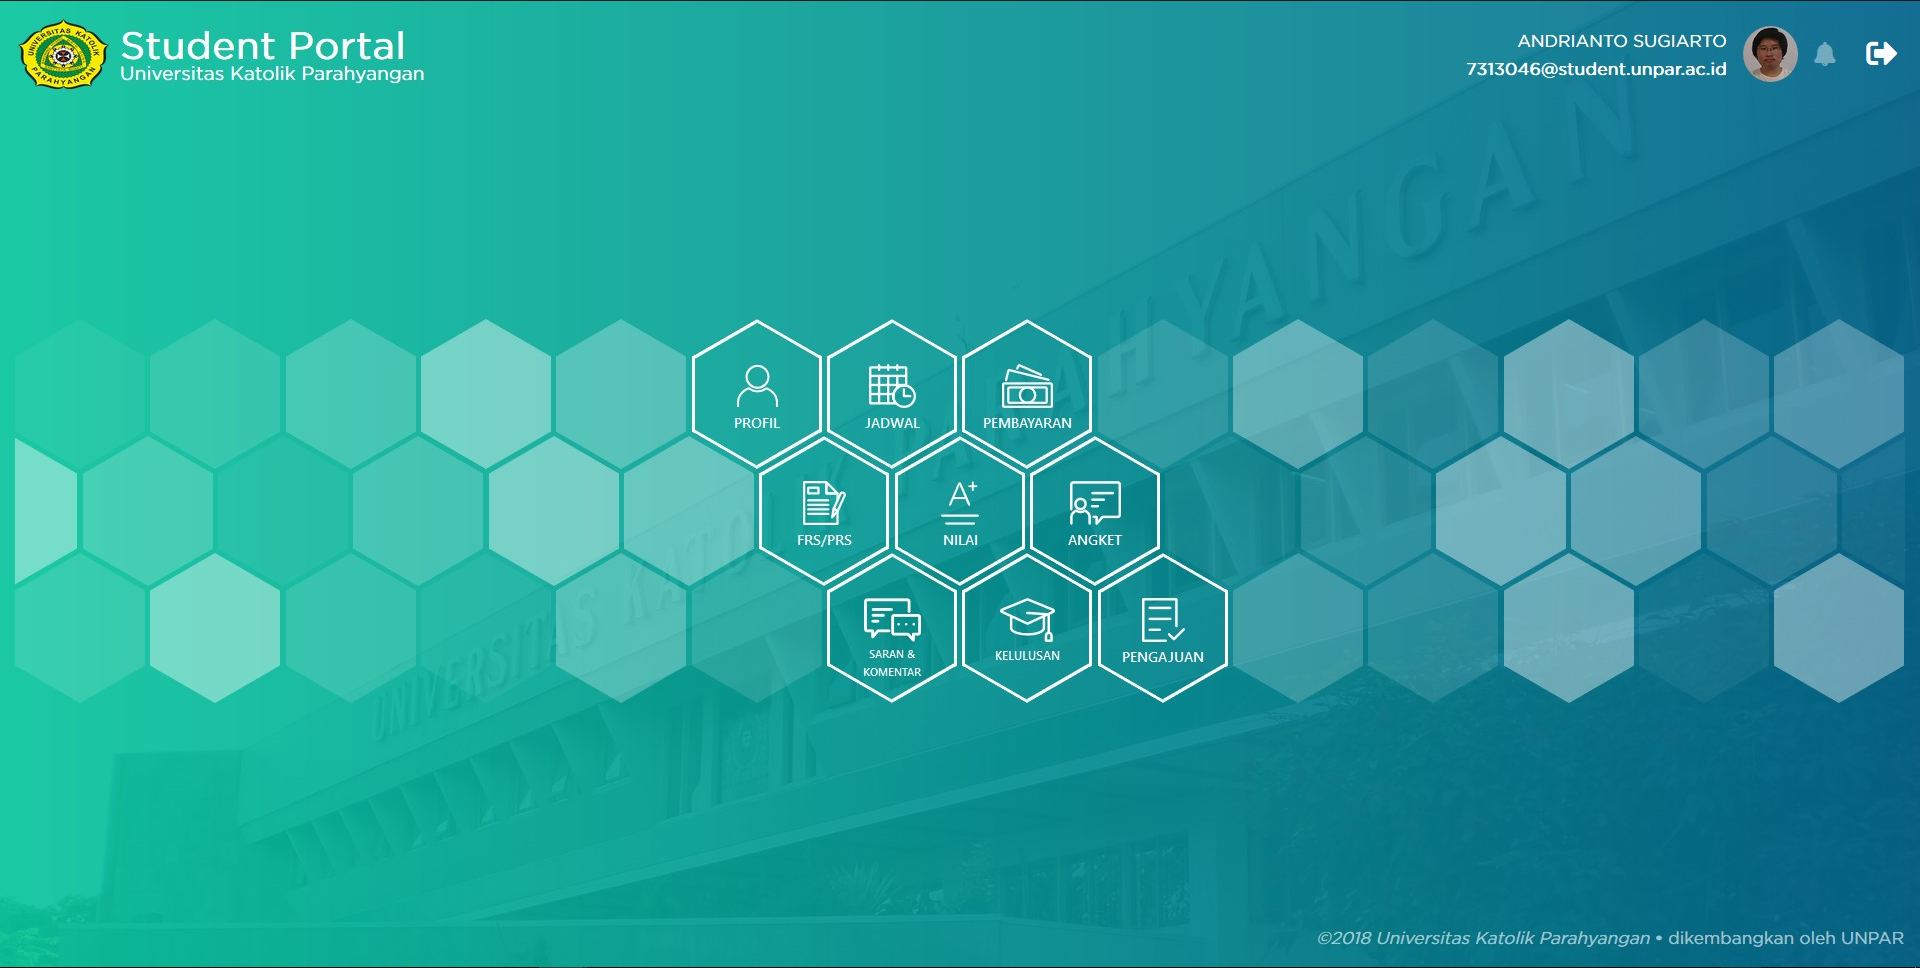
\includegraphics[scale=0.3]{Gambar/studentportal_home}
		\caption{Halaman Utama Portal Akademik Mahasiswa}
		\label{fig:studentportal_home}
	\end{figure}
	\item Menu Student Portal \\
	Bagian ini memuat fitur-fitur Student Portal yang terdiri dari:
	\begin{itemize}
		\item \textbf{Profil}, berisi tentang data diri masing-masing mahasiswa (Gambar \ref{fig:studentportal_profil}).
		\begin{figure}[H]
		\centering
		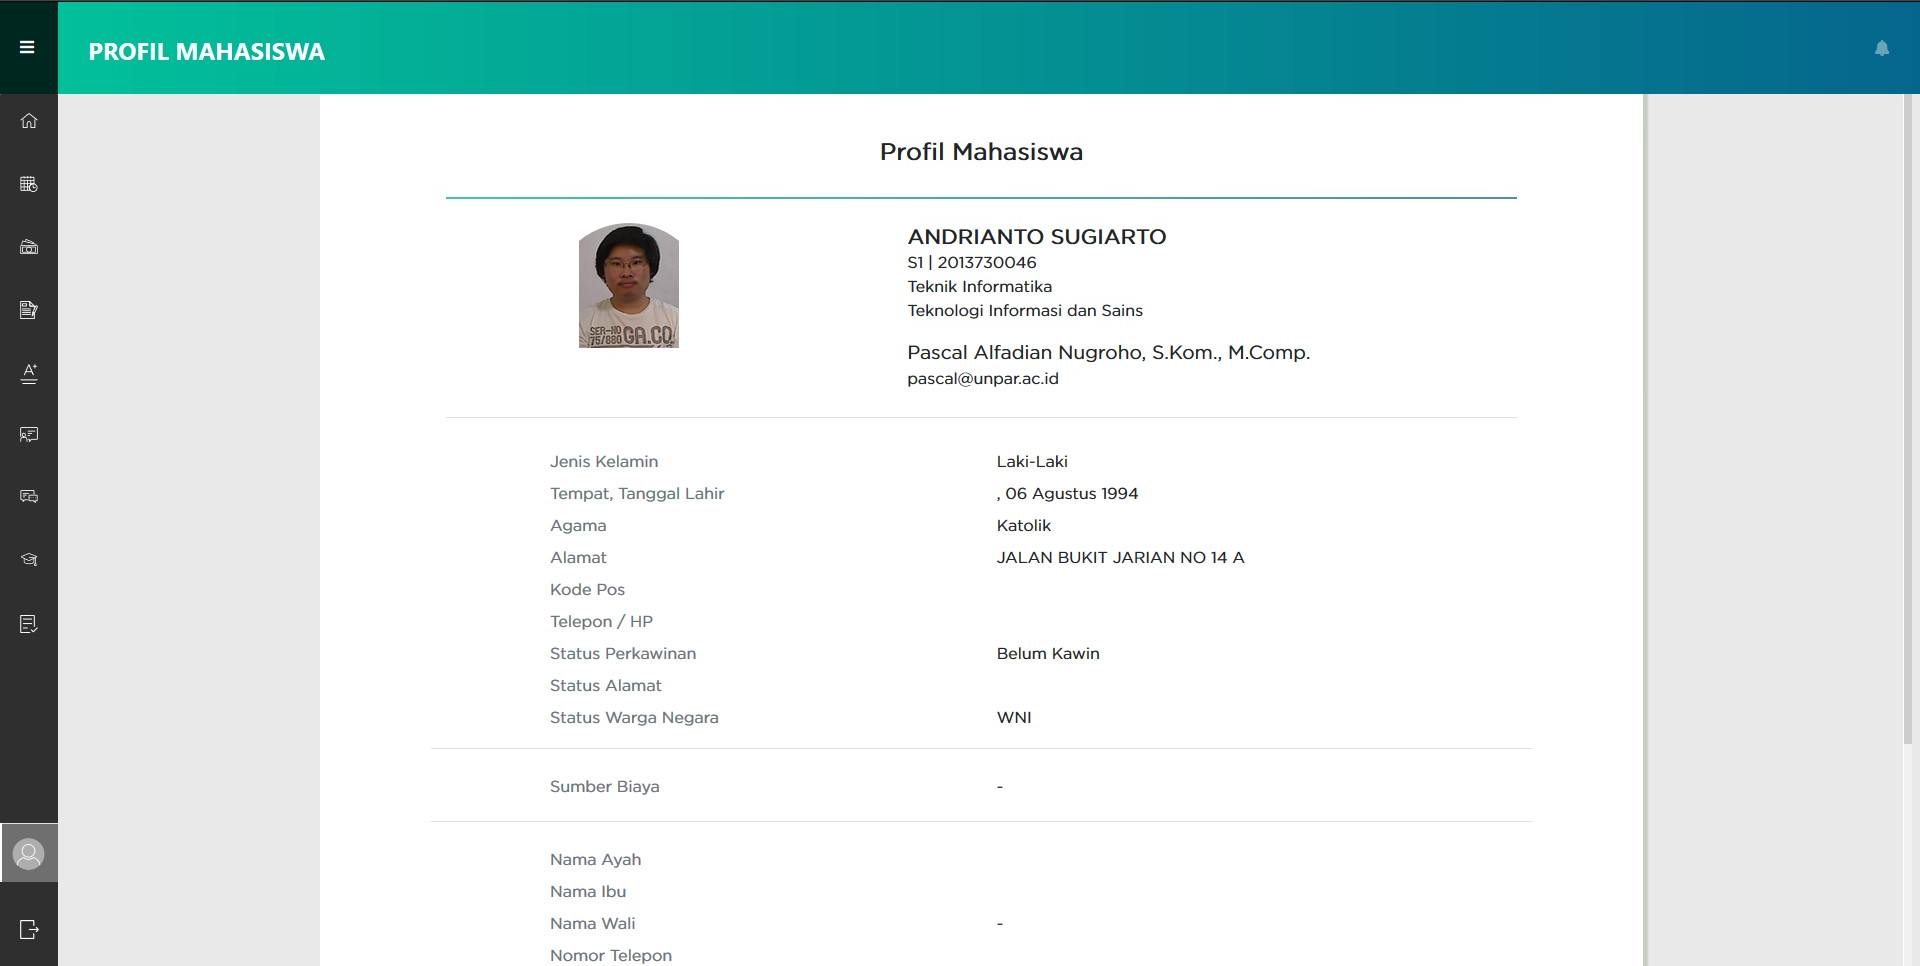
\includegraphics[scale=0.3]{Gambar/studentportal_profil}
		\caption{Tampilan Profil Student Portal}
		\label{fig:studentportal_profil}
		\end{figure}
		\item \textbf{Jadwal} \\
		Menu Jadwal terdiri dari submenu:
		\begin{itemize}
			\item Kuliah \\
			Submenu ini berisi tentang jadwal kuliah yang dapat disusun per semester dan terdapat 2 tampilan, yaitu tabel waktu dan tabel biasa (Gambar \ref{fig:studentportal_jadwal_kuliah_timetable} \& \ref{fig:studentportal_jadwal_kuliah_table})
			\begin{figure}[H]
			\centering
			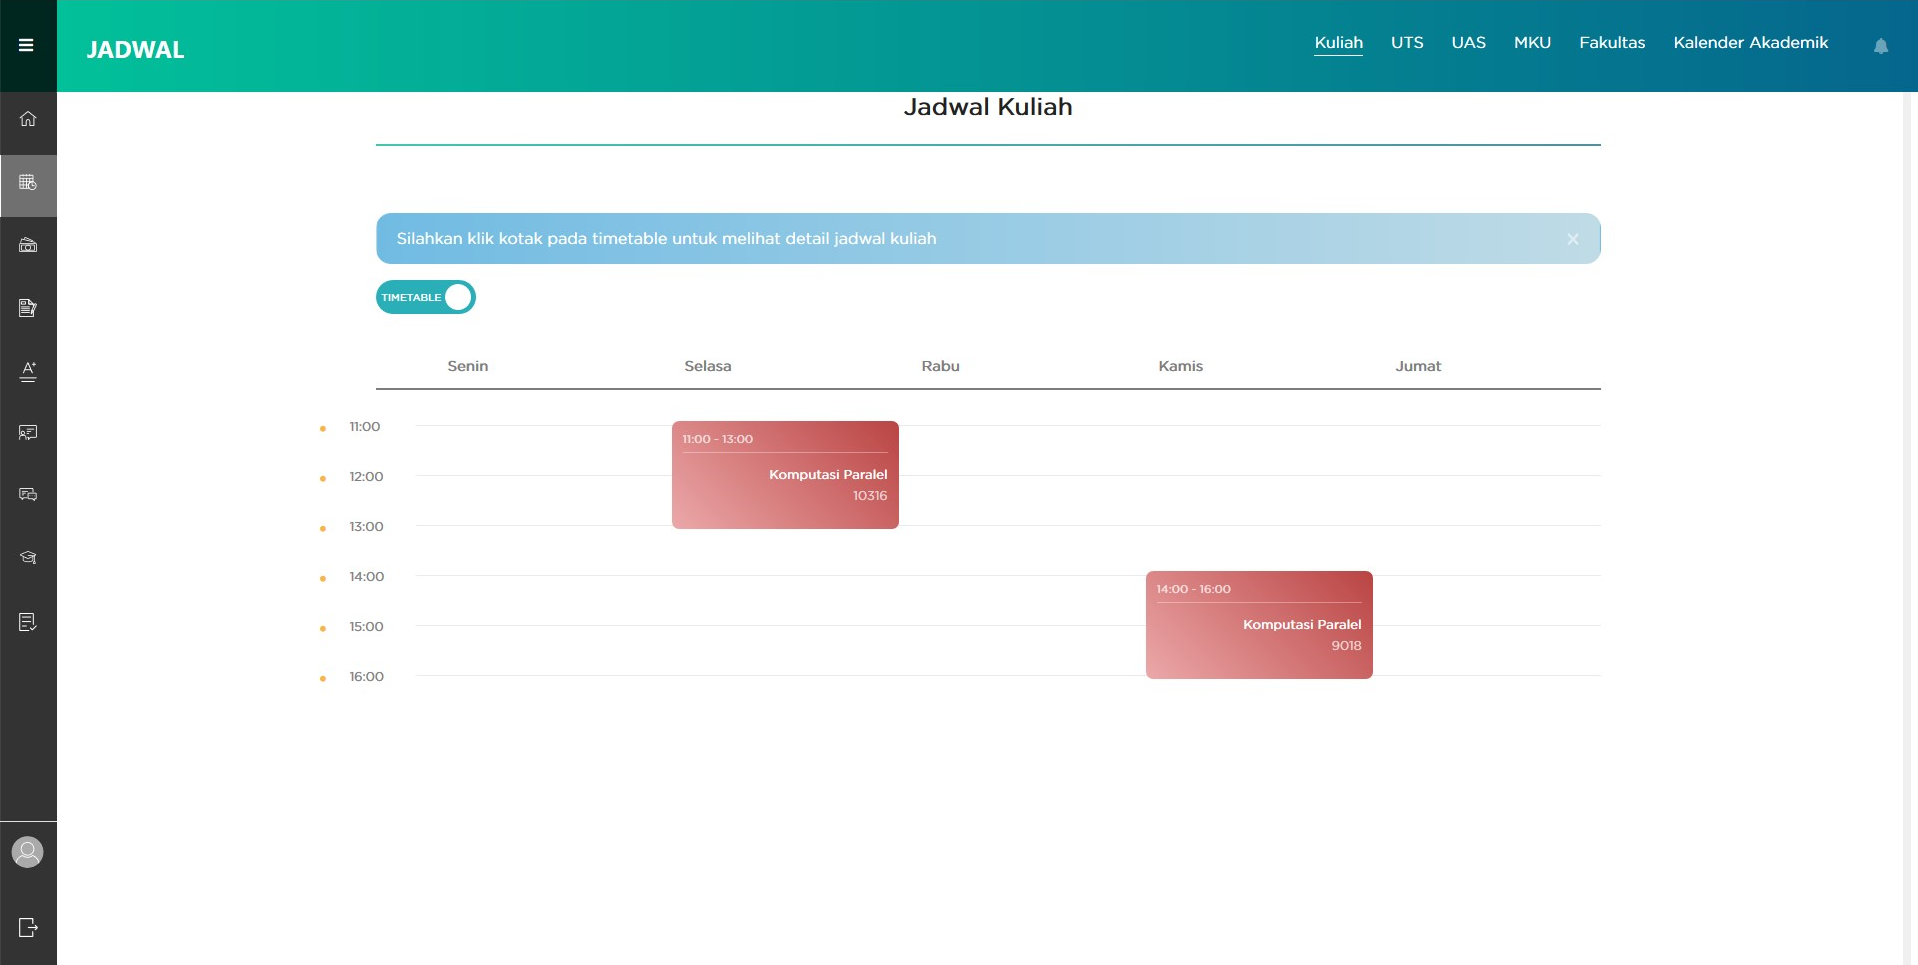
\includegraphics[scale=0.3]{Gambar/studentportal_jadwal_kuliah}
			\caption{Tampilan Jadwal Kuliah Dalam Tabel Waktu}
			\label{fig:studentportal_jadwal_kuliah_timetable}
			\end{figure}
			\begin{figure}[H]
			\centering
			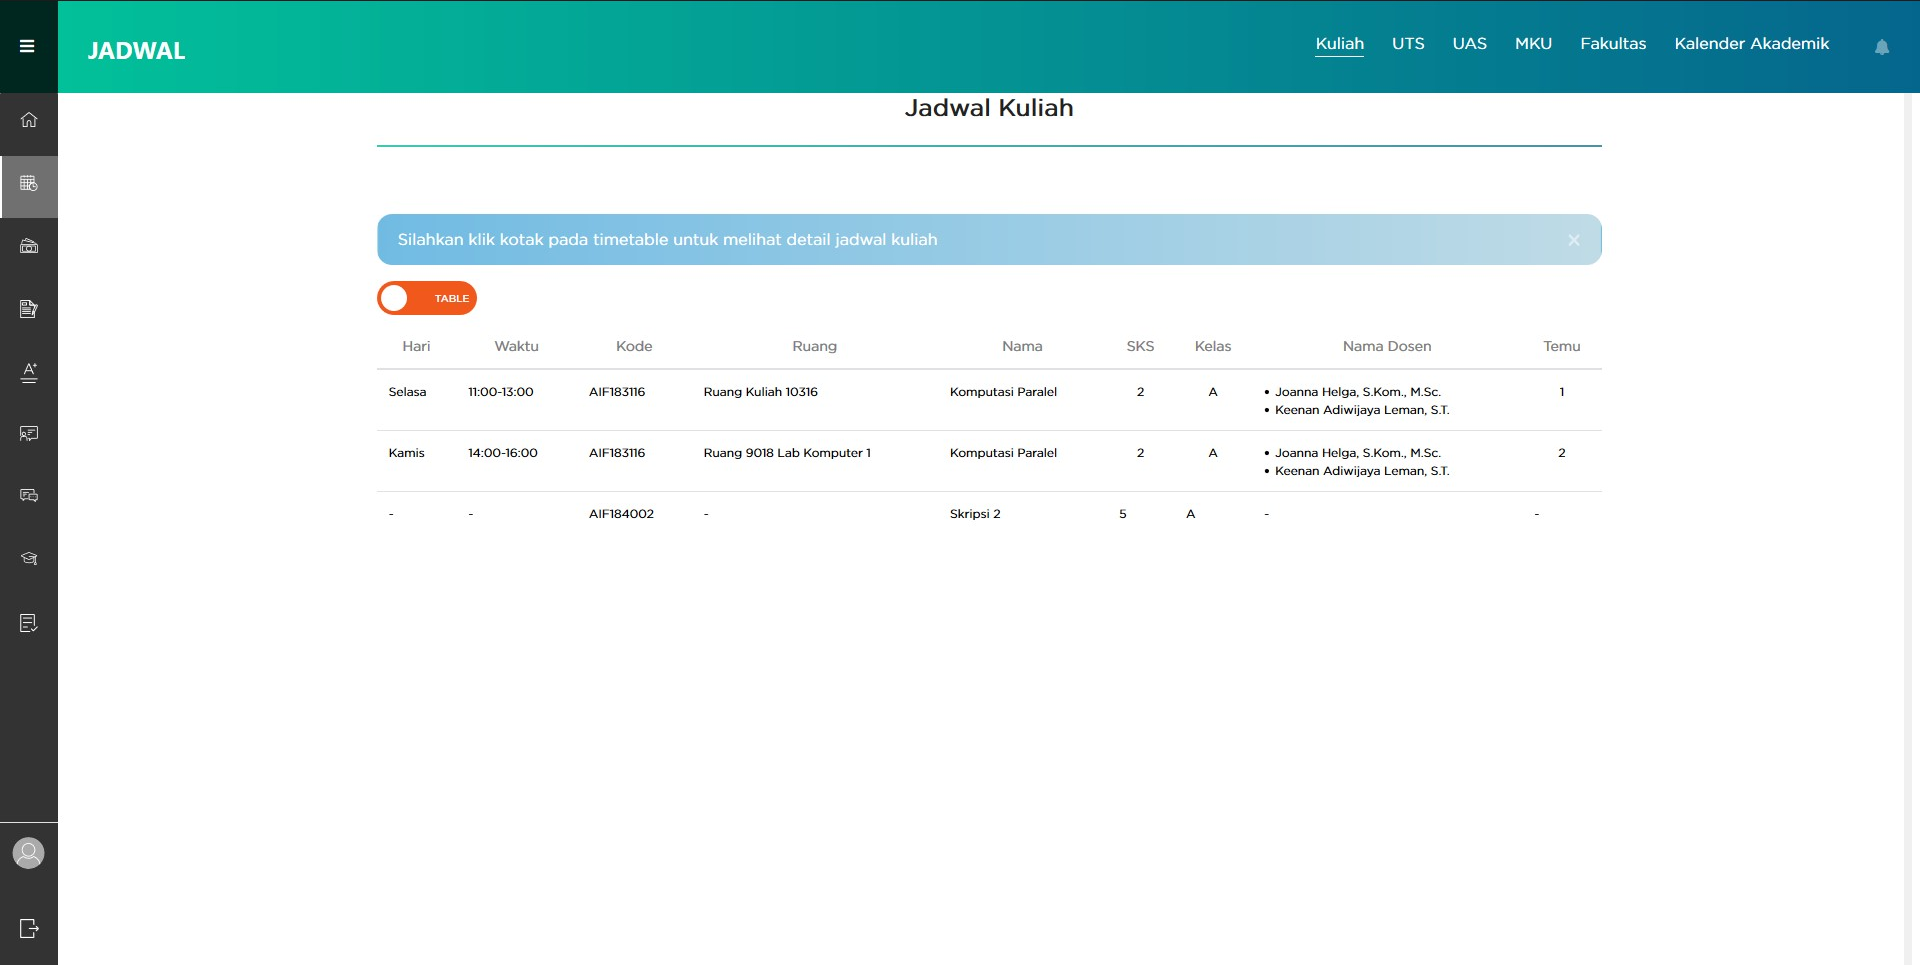
\includegraphics[scale=0.3]{Gambar/studentportal_jadwal_kuliah_table}
			\caption{Tampilan Jadwal Kuliah Tabel}
			\label{fig:studentportal_jadwal_kuliah_table}
			\end{figure}
			\item UTS \\
			Submenu ini berisi tentang UTS yang dapat disusun per semester (Gambar \ref{fig:studentportal_uts})
			\begin{figure}[H]
			\centering
			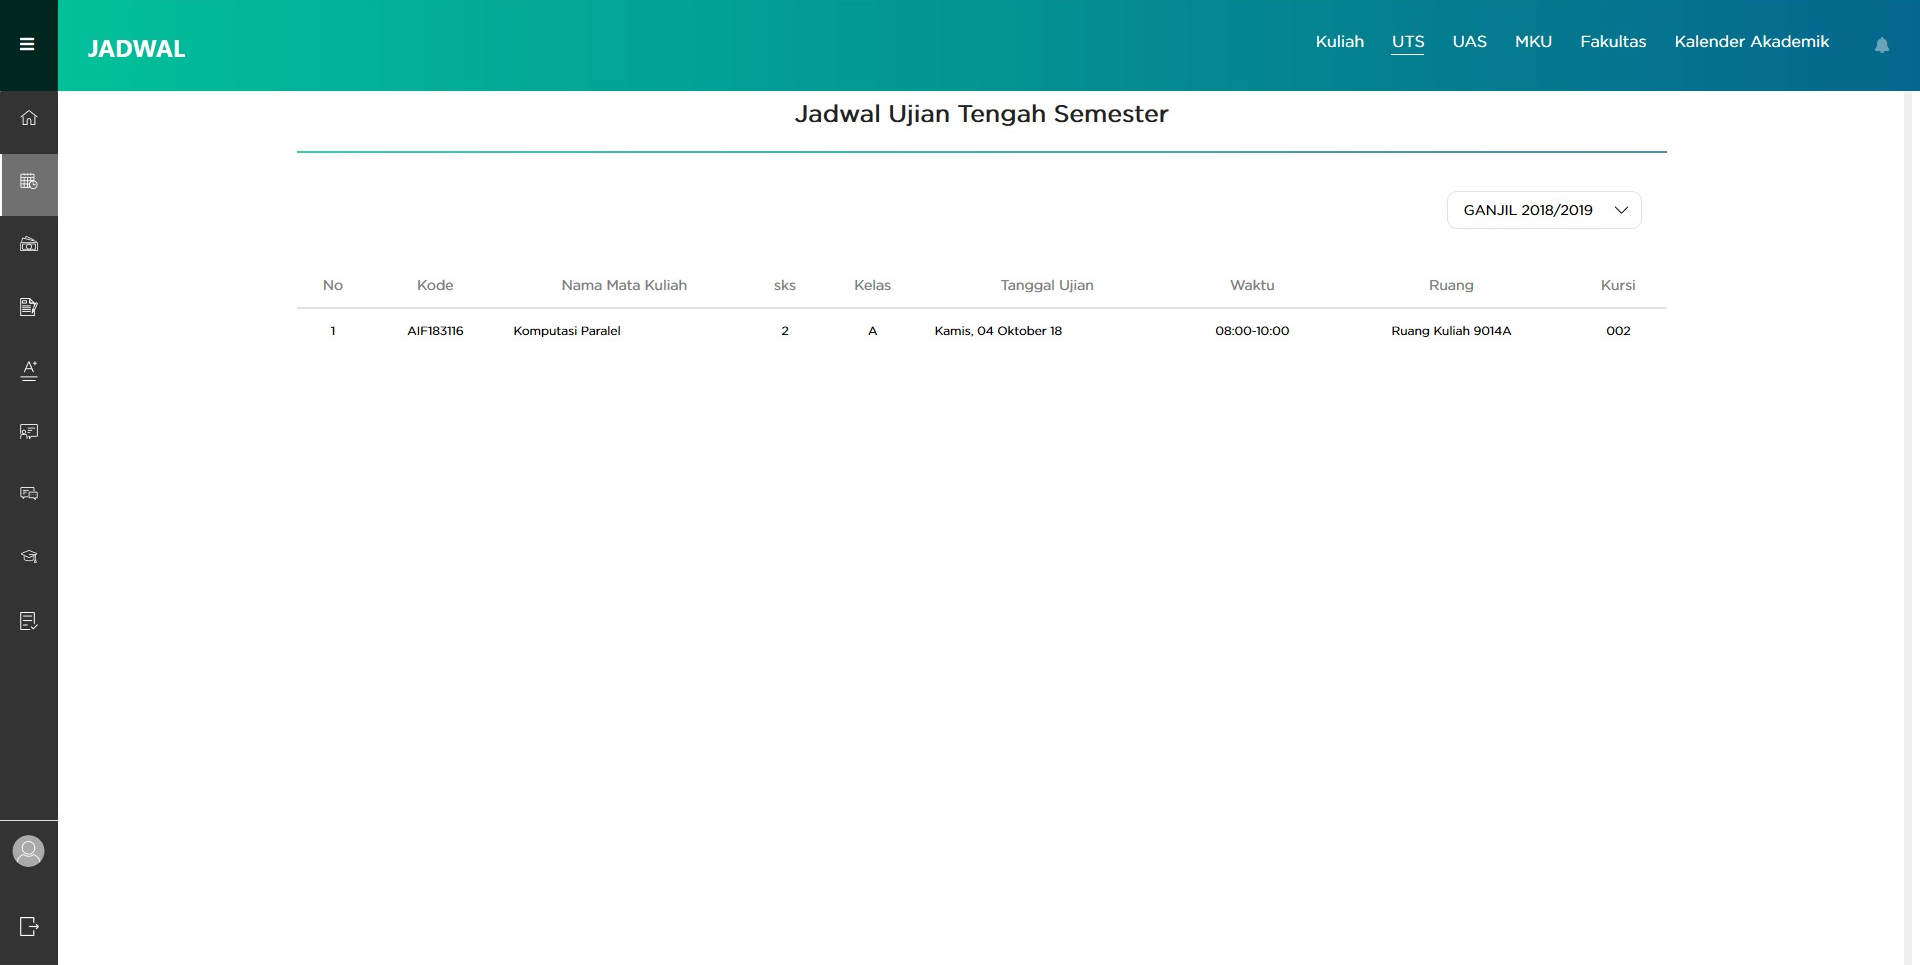
\includegraphics[scale=0.3]{Gambar/studentportal_jadwal_uts}
			\caption{Tampilan UTS}
			\label{fig:studentportal_uts}
			\end{figure}
			\item UAS \\
			Submenu ini berisi tentang UAS yang dapat disusun per semester (Gambar \ref{fig:studentportal_uas})
			\begin{figure}[H]
			\centering
			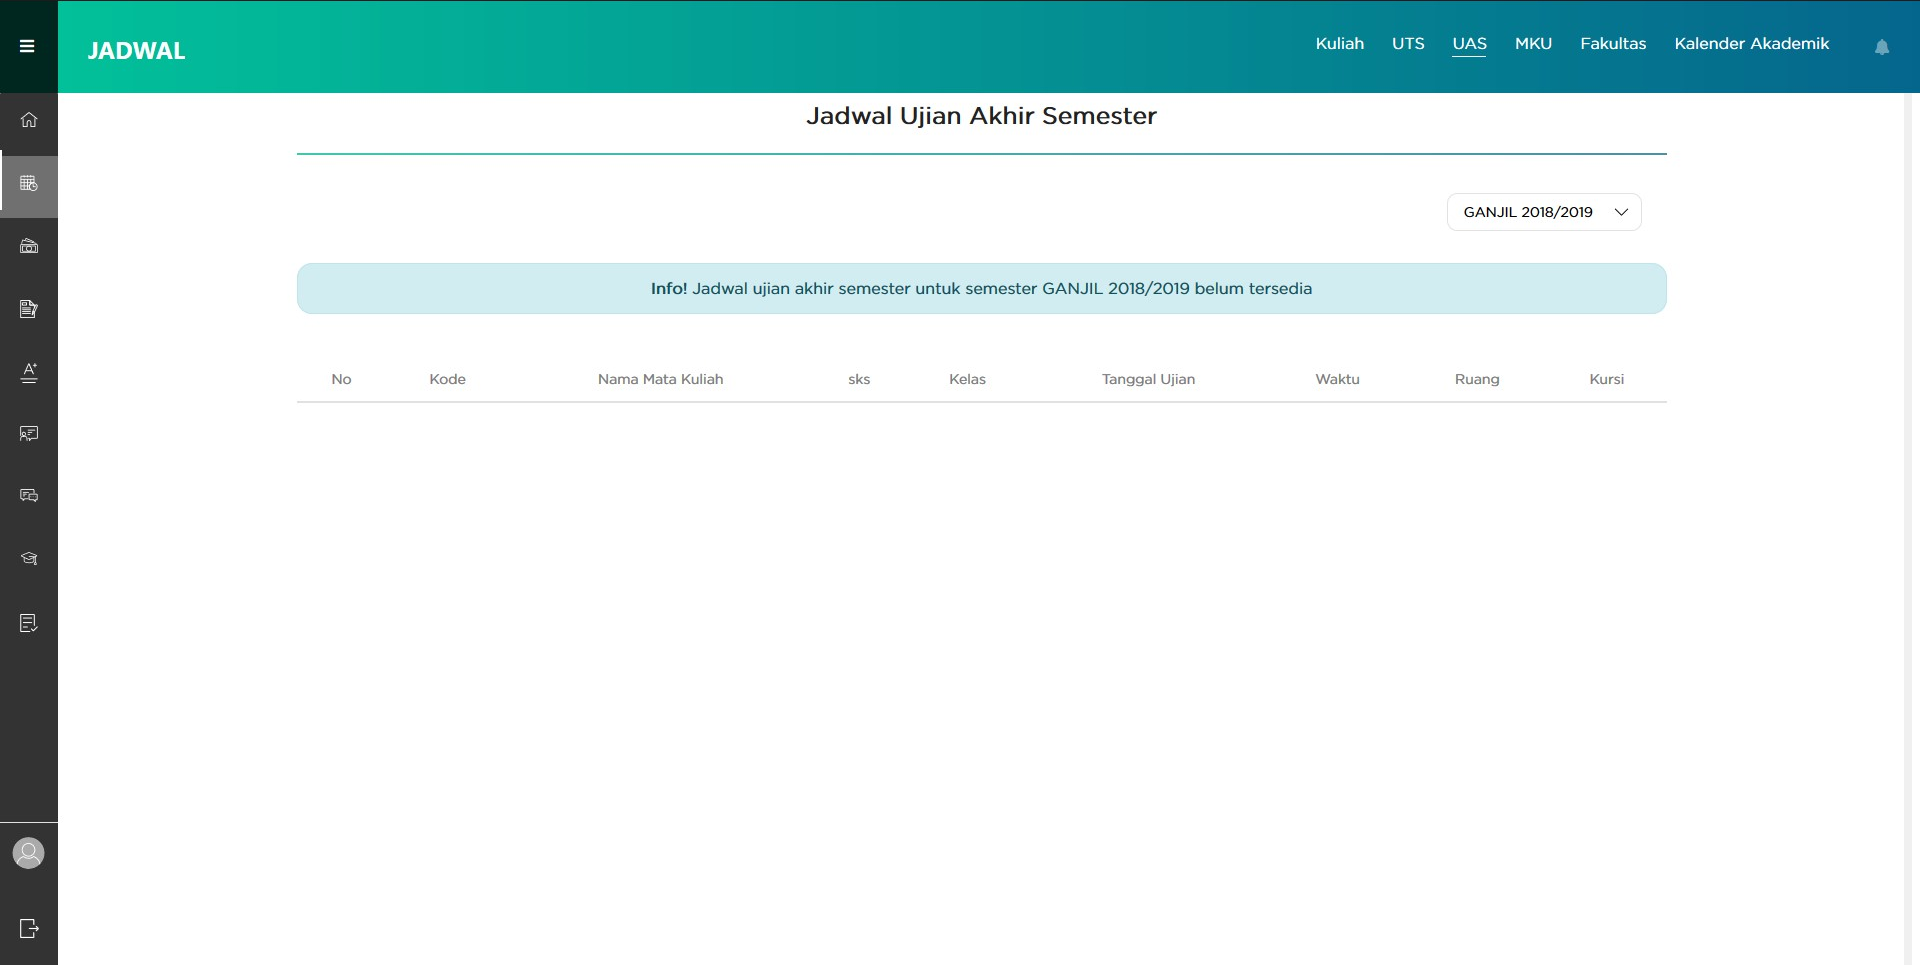
\includegraphics[scale=0.3]{Gambar/studentportal_jadwal_uas}
			\caption{Tampilan UAS}
			\label{fig:studentportal_uas}
			\end{figure}
			\item MKU \\
			Submenu ini menampilkan seluruh jadwal Mata Kuliah Umum (MKU) yang memberikan informasi tentang kelas-kelas yang dibuka oleh Pusat Kajian Humaniora (PKH) (Gambar \ref{fig:studentportal_jadwal_mku})
			\begin{figure}[H]
			\centering
			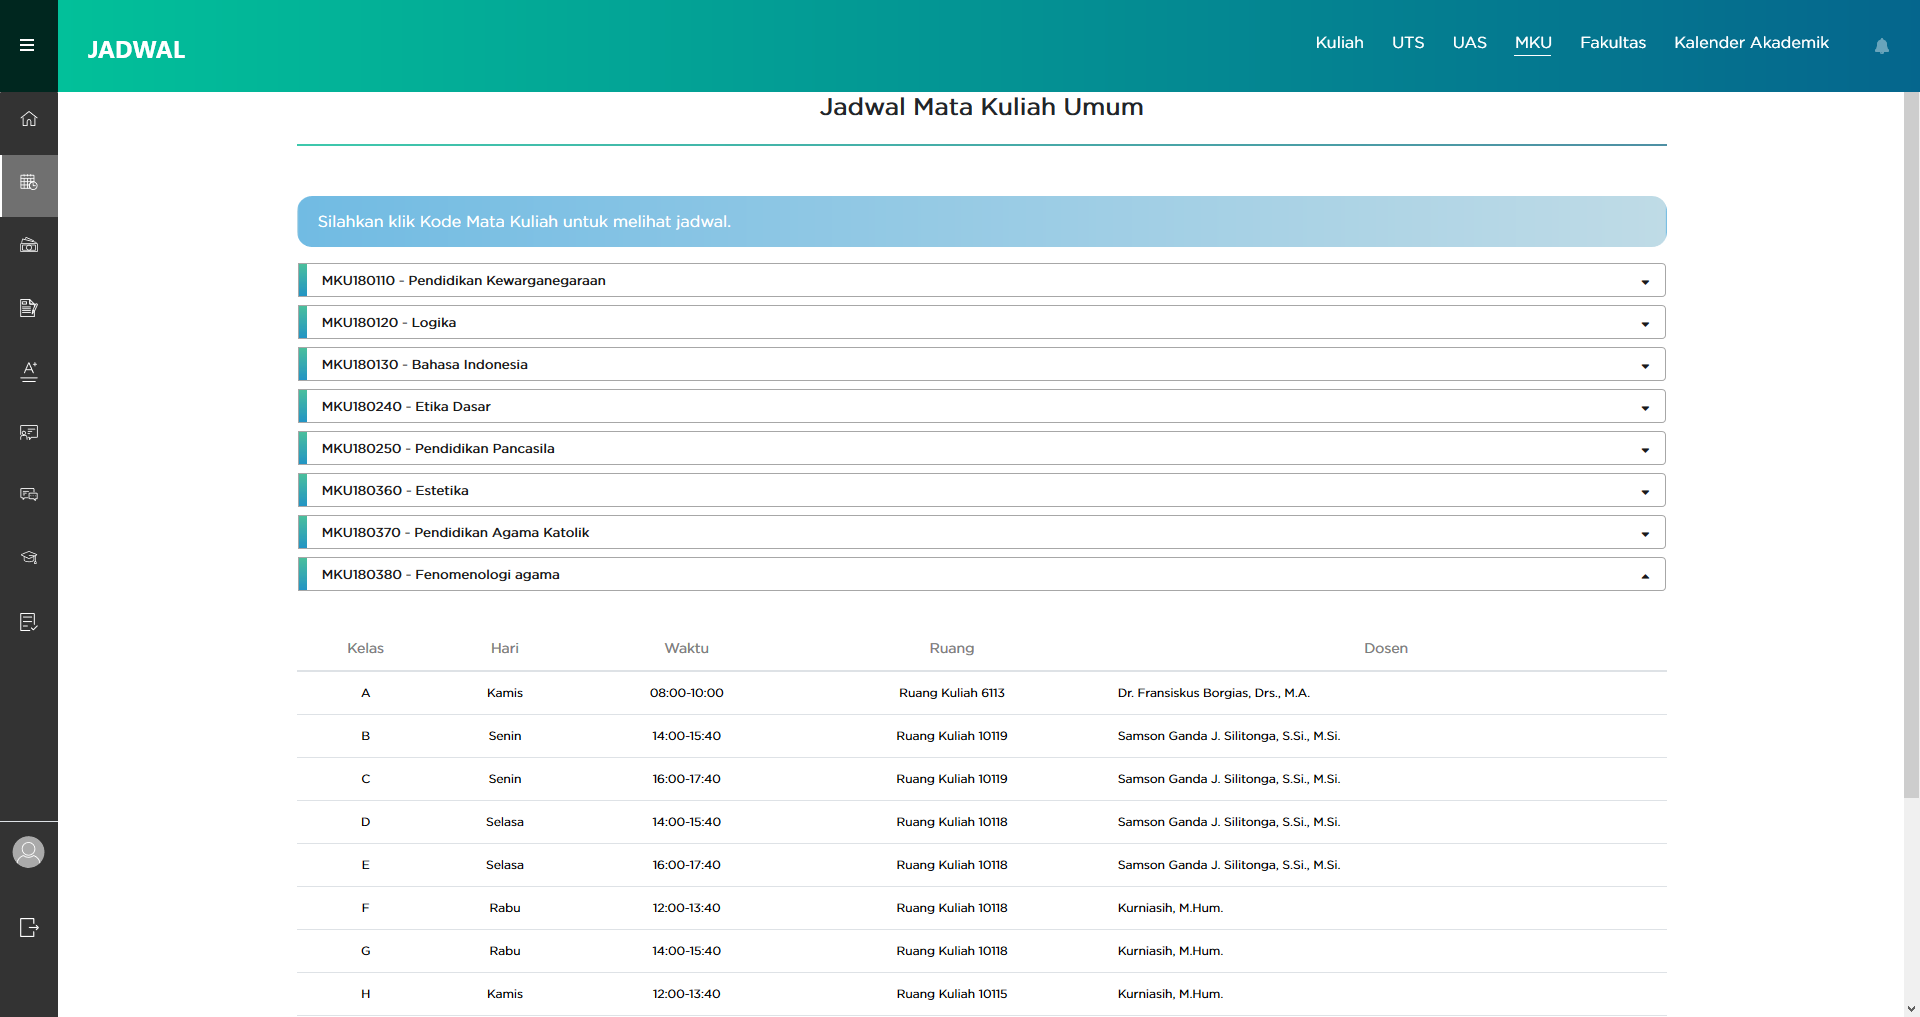
\includegraphics[scale=0.23]{Gambar/studentportal_jadwal_mku}
			\caption{Tampilan MKU}
			\label{fig:studentportal_jadwal_mku}
			\end{figure}
			\item Seluruh Fakultas \\
			Submenu ini memberikan informasi mengenai jadwal-jadwal yang ada diseluruh fakultas dan masih dalam pembangunan (Gambar \ref{fig:studentportal_jadwal_seluruh_fakultas})
			\begin{figure}[H]
			\centering
			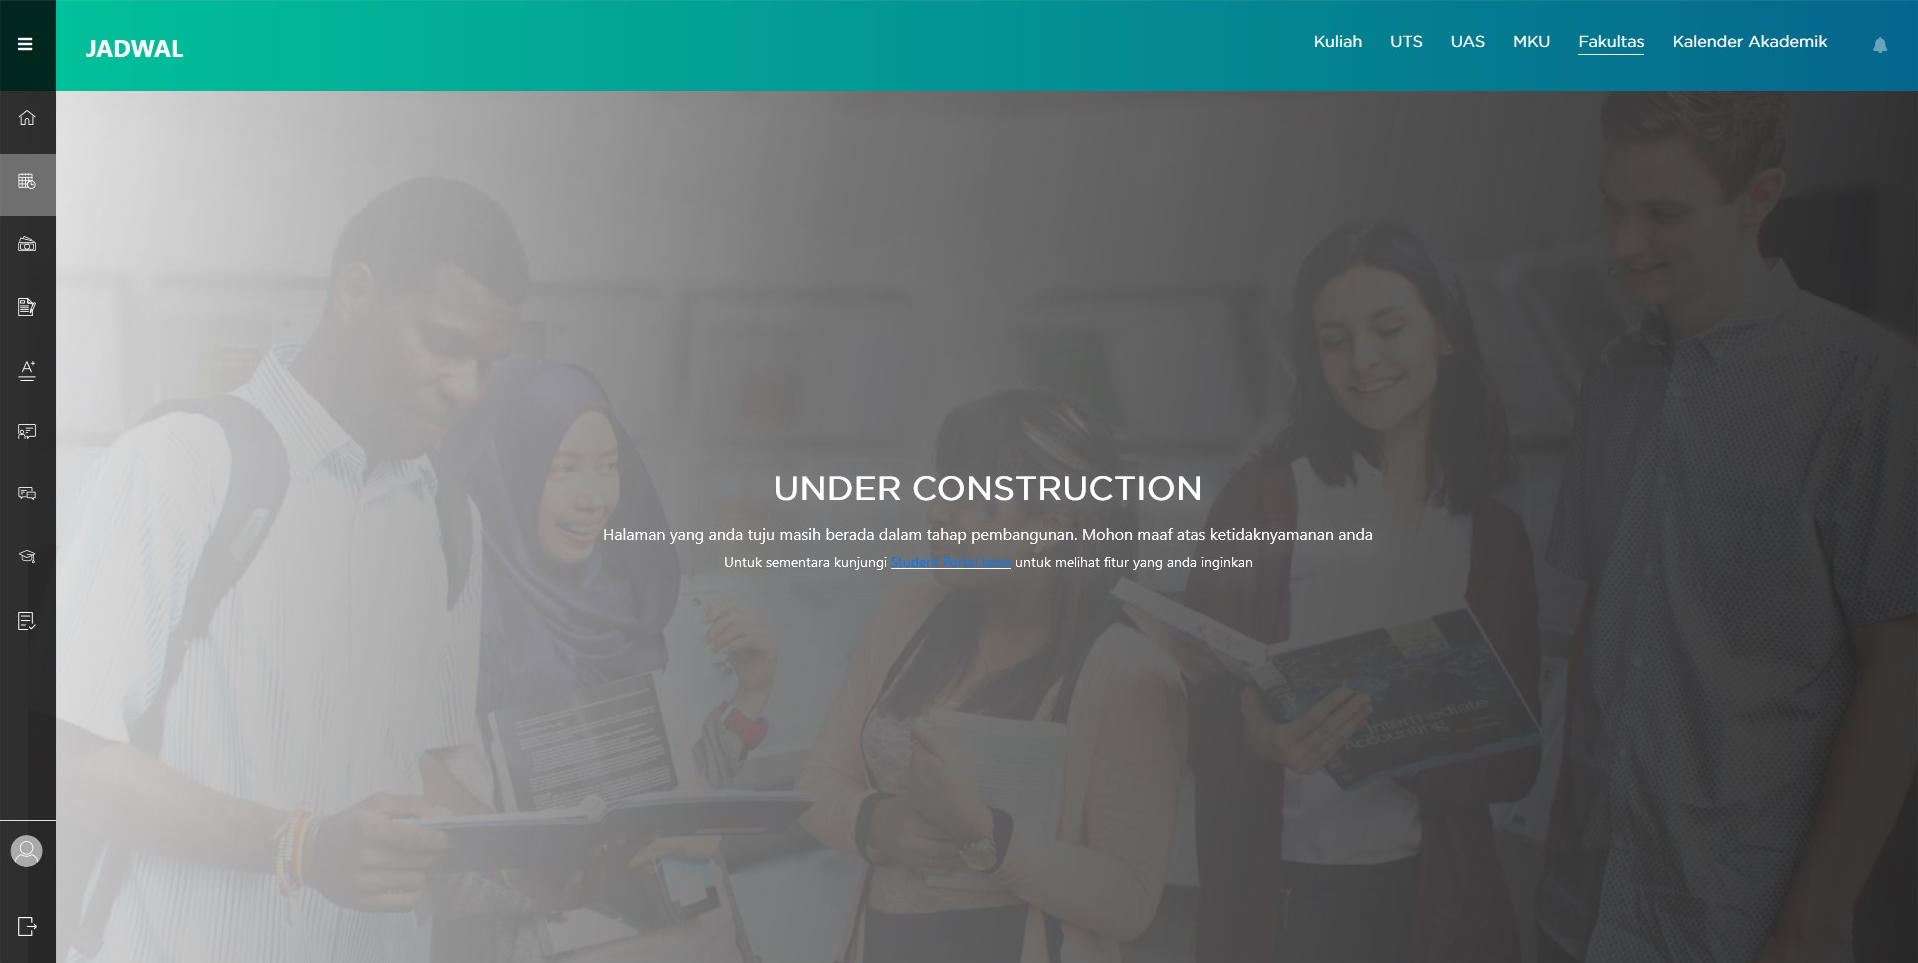
\includegraphics[scale=0.3]{Gambar/studentportal_seluruh_fakultas_under_construction}
			\caption{Tampilan Jadwal Seluruh Fakultas Under Construction}
			\label{fig:studentportal_jadwal_seluruh_fakultas}
			\end{figure}
			\item Kalender Akademik \\
			Submenu ini memberikan informasi kalender akademik UNPAR dan masih dalam pembangunan.
		\end{itemize}
		\item \textbf{Pembayaran Uang Kuliah} \\
		Menu ini berfungsi untuk melihat data tagihan pembayaran uang kuliah, riwayat pembayaran, dan keterangan cara-cara pembayaran uang kuliah (Gambar \ref{fig:studentportal_pembayaran_kuliah}).
		\begin{figure}[H]
			\centering
			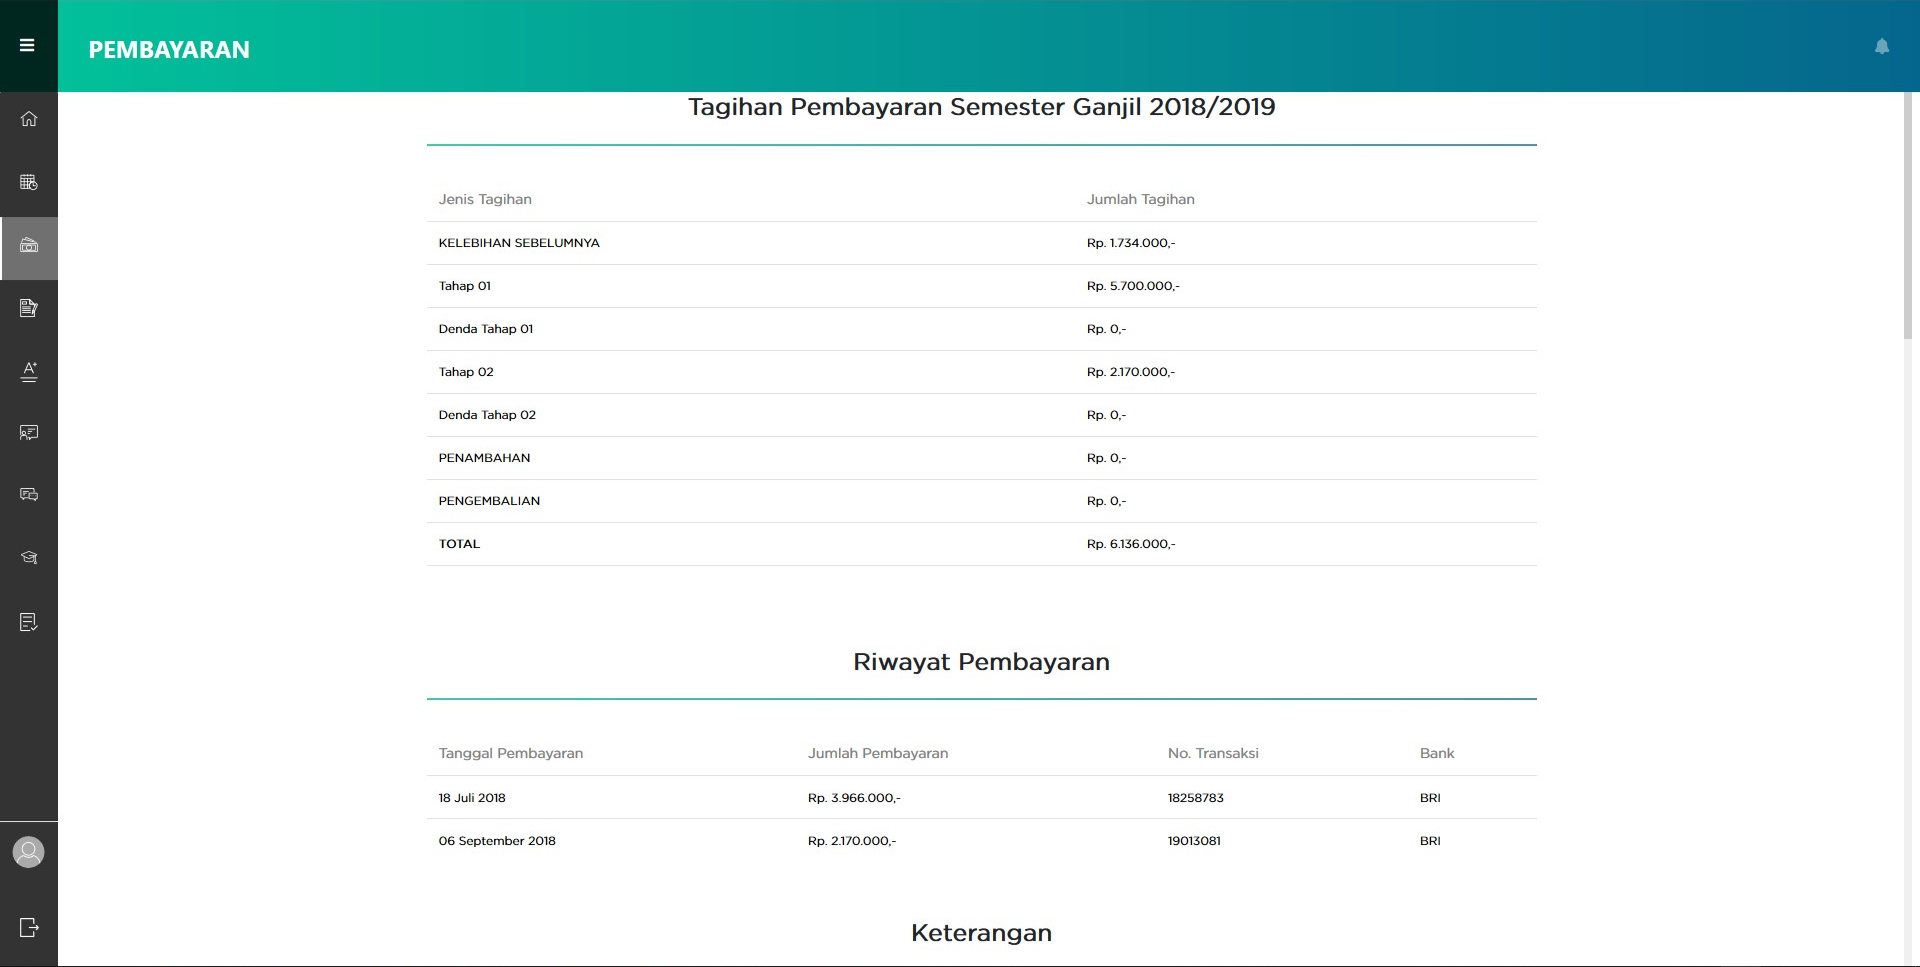
\includegraphics[scale=0.3]{Gambar/studentportal_pembayaran_kuliah}
			\caption{Tampilan Pembayaran Kuliah}
			\label{fig:studentportal_pembayaran_kuliah}
		\end{figure}
		\item FRS/PRS
		Menu FRS/PRS terdiri dari submenu:
		\begin{itemize}
			\item FRS/PRS \\
			Digunakan sebagai formulir pengisian rencana studi awal (FRS), perubahan rencana studi(PRS) dan menampilkan informasi mata kuliah yang telah diambil saat FRS atau PRS (Gambar \ref{fig:studentportal_frs_prs}).
			\begin{figure}[H]
				\centering
				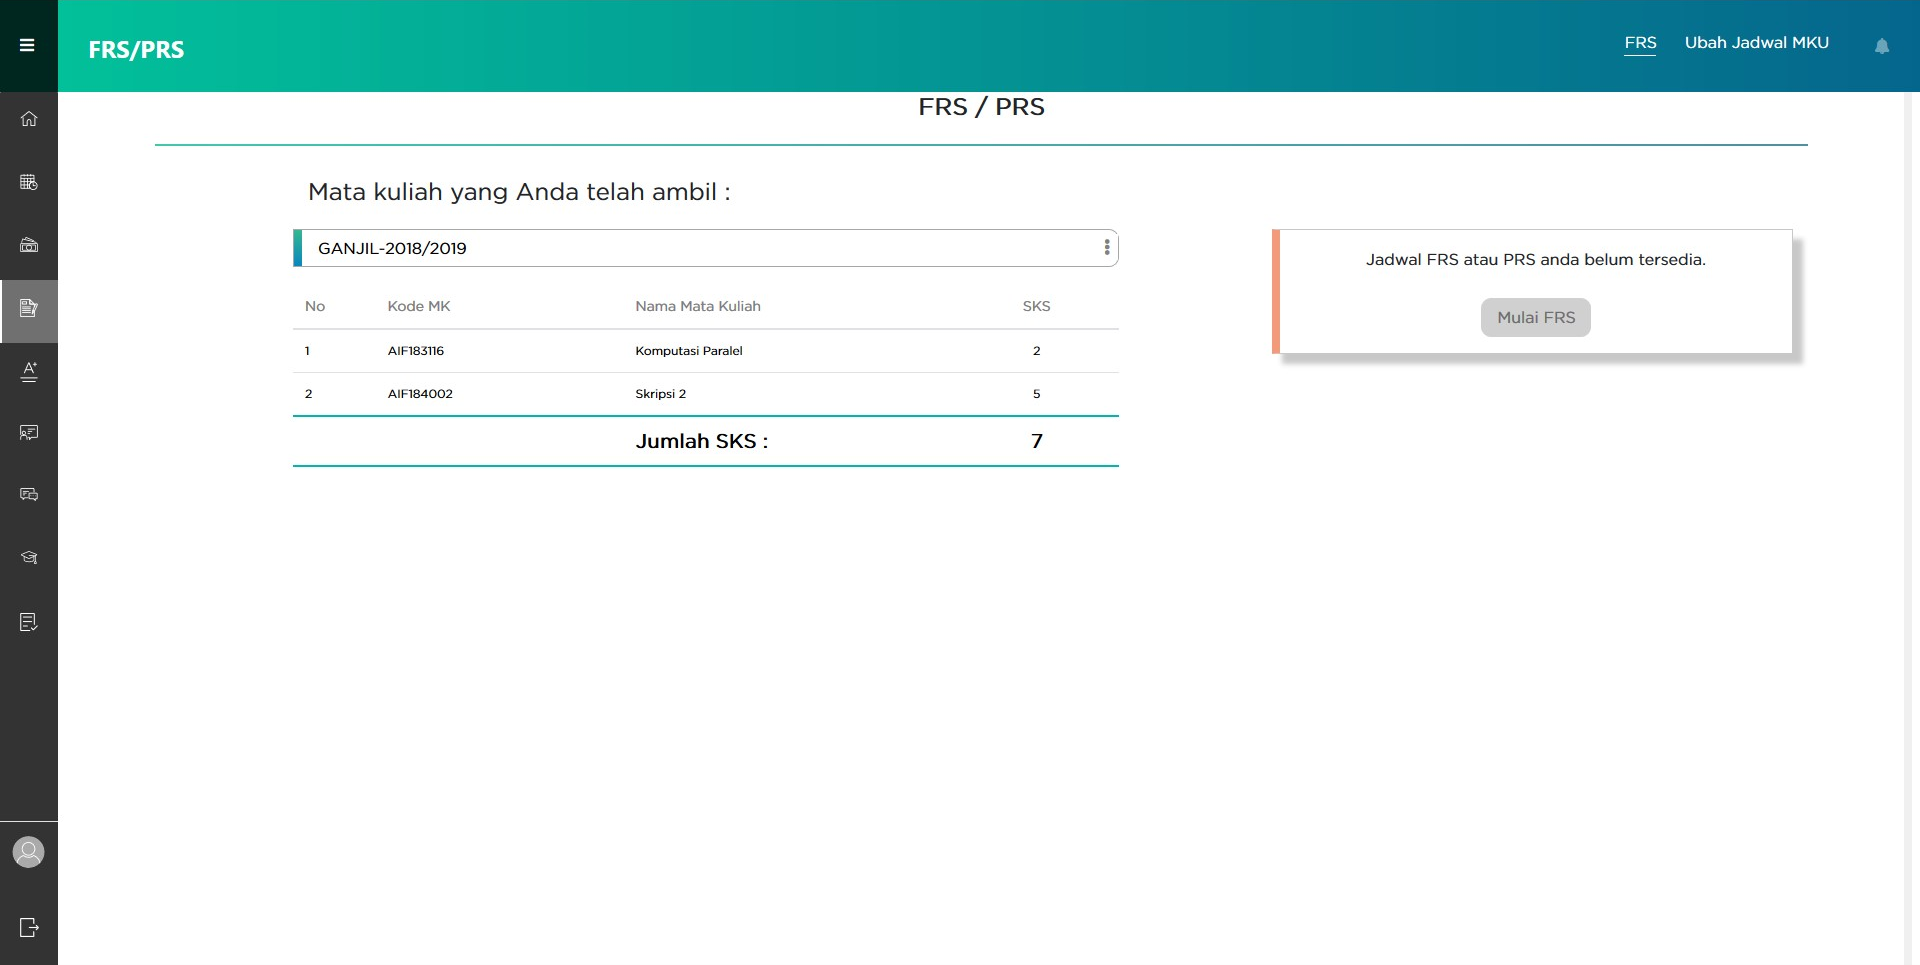
\includegraphics[scale=0.3]{Gambar/studentportal_frs_prs}
				\caption{Tampilan FRS/PRS}
				\label{fig:studentportal_frs_prs}
			\end{figure}
			\item Ubah Jadwal MKU \\
			Mahasiswa dapat mengubah jadwal kelas MKU (Gambar \ref{fig:studentportal_ubah_jadwal_mku}).
			\begin{figure}[H]
				\centering
				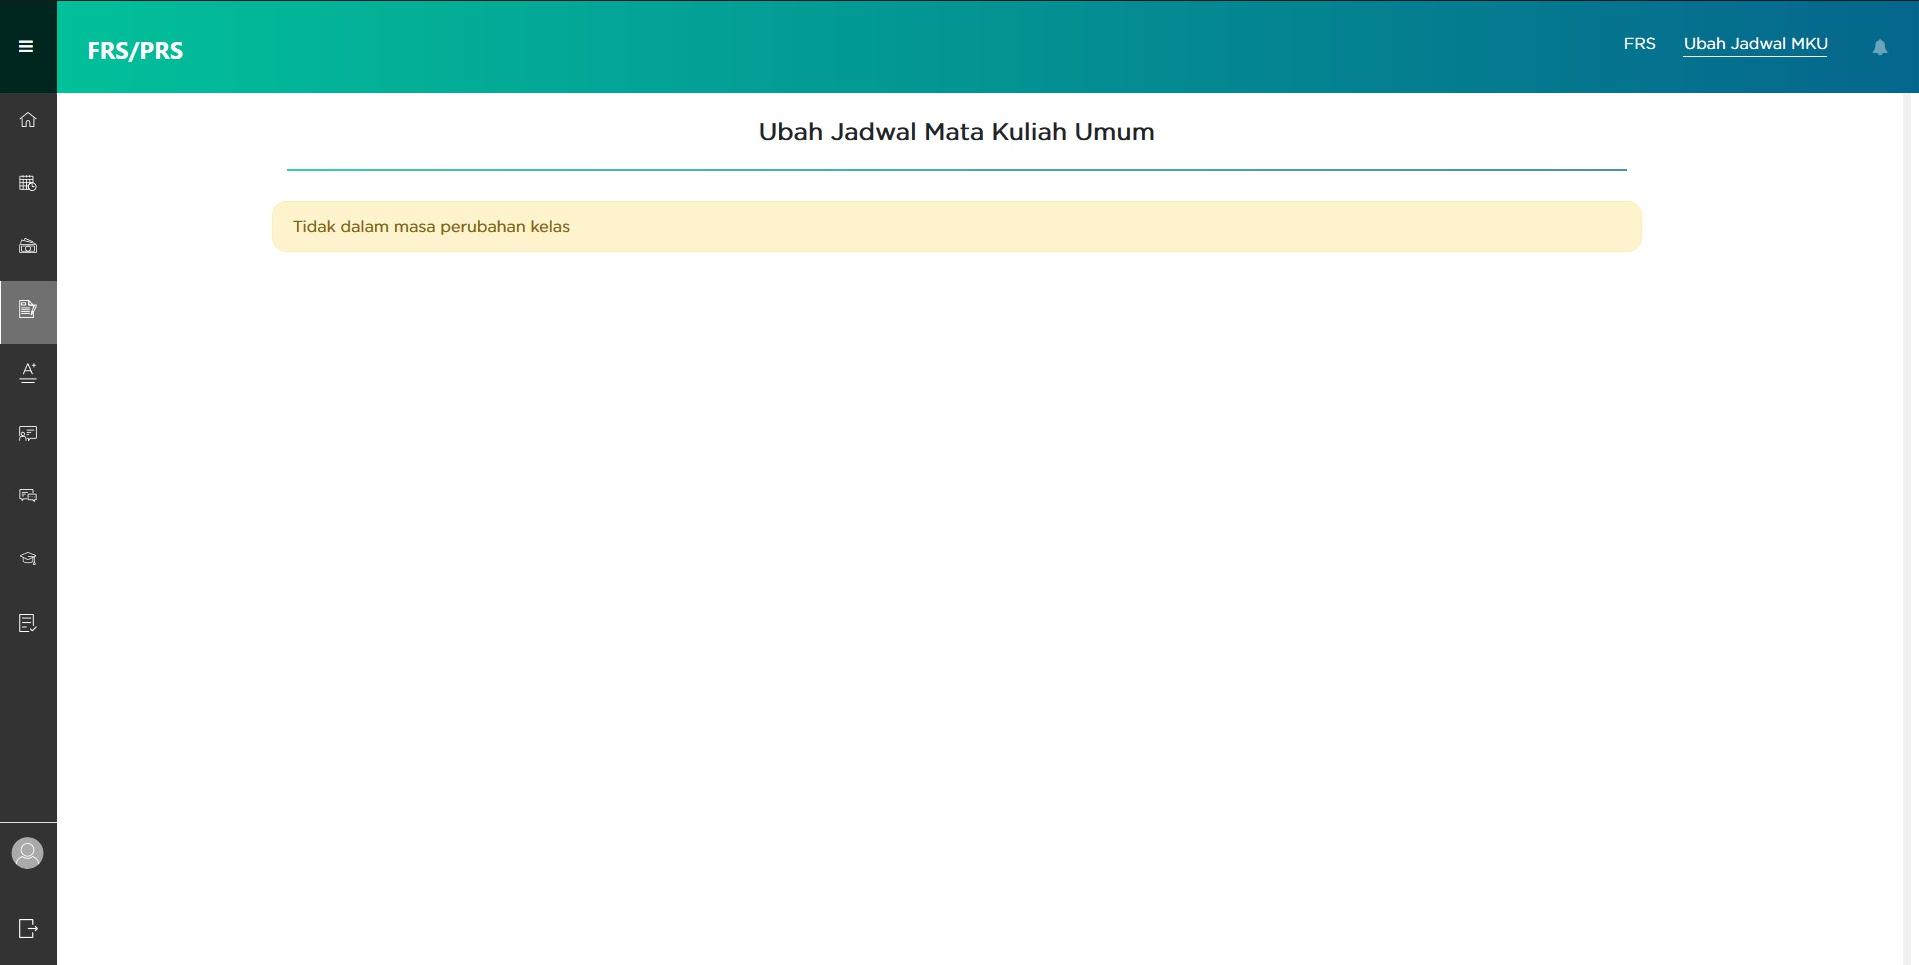
\includegraphics[scale=0.3]{Gambar/studentportal_ubah_jadwal_mku}
				\caption{Tampilan Ubah Jadwal MKU}
				\label{fig:studentportal_ubah_jadwal_mku}
			\end{figure}
		\end{itemize}
		\item \textbf{Nilai}
		Menu Nilai terdiri dari submenu:
		\begin{itemize}
			\item Nilai per Semester \\
			Submenu ini menampilkan informasi nilai per semester. Mahasiswa dapat melihat nilai sesuai dengan semester yang dipilih (Gambar \ref{fig:studentportal_nilai_per_semesters}).
			\begin{figure}[H]
				\centering
				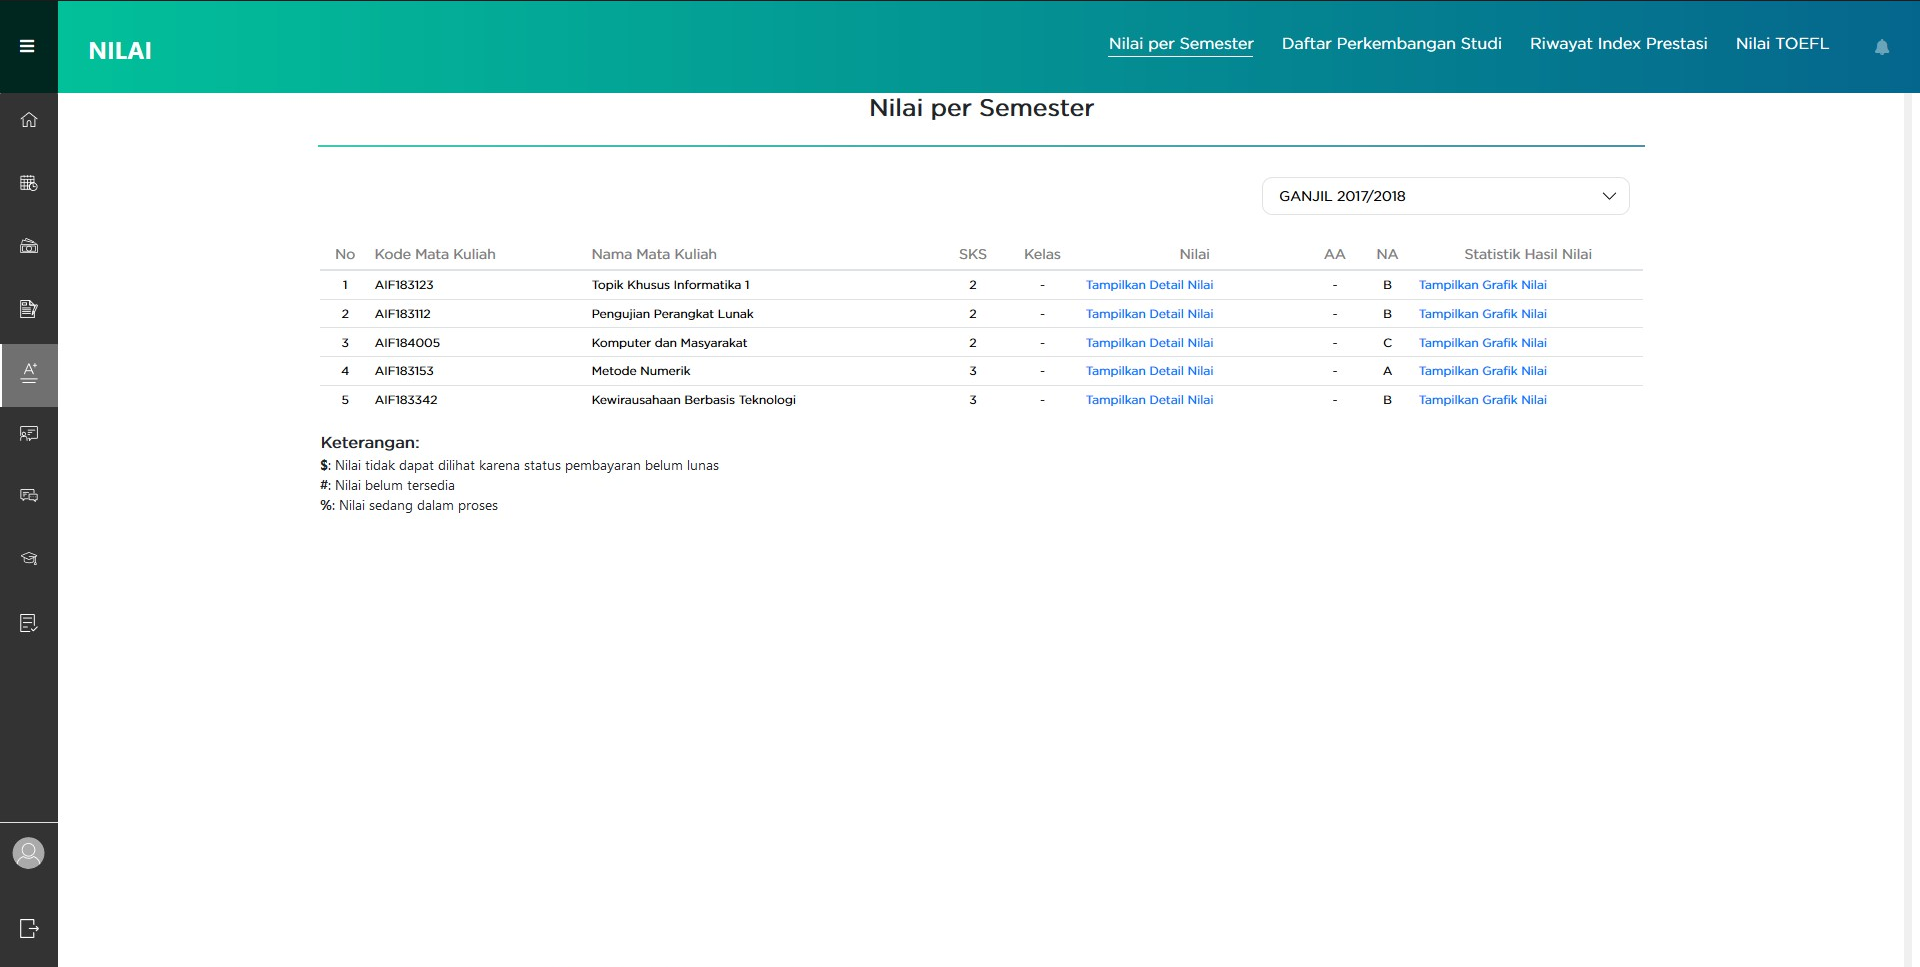
\includegraphics[scale=0.3]{Gambar/studentportal_nilai_per_semester}
				\caption{Tampilan Nilai Per Semester}
				\label{fig:studentportal_nilai_per_semester}
			\end{figure}
			\item Daftar Perkembangan Studi \\
			Seluruh riwayat mata kuliah dan nilai yang pernah ditempuh di submenu ini (Gambar \ref{fig:studentportal_dps_1}). Pada bagian bawah halaman, terdapat statistik nilai dan indeks perstasi (Gambar \ref{fig:studentportal_dps_2}).
			\begin{figure}[H]
				\centering
				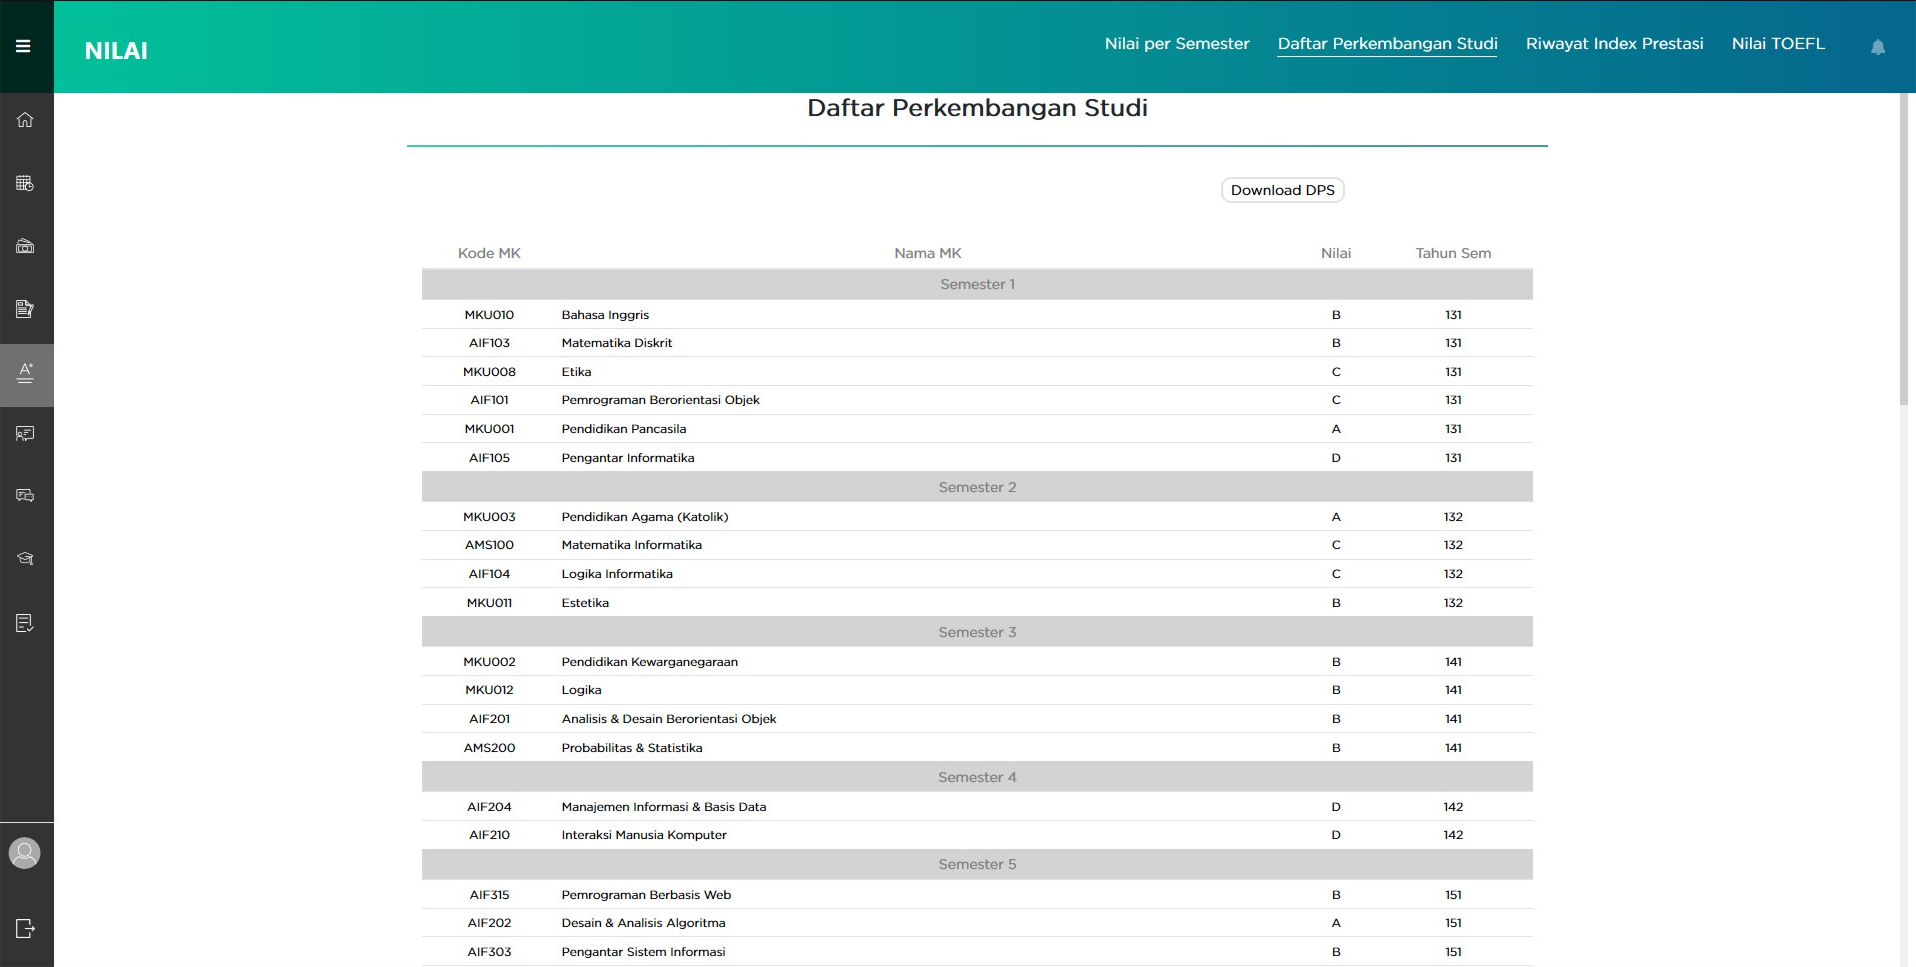
\includegraphics[scale=0.3]{Gambar/studentportal_dps_1}
				\caption{Tampilan Daftar Perkembangan Studi}
				\label{fig:studentportal_dps_1}
			\end{figure}
			\begin{figure}[H]
				\centering
				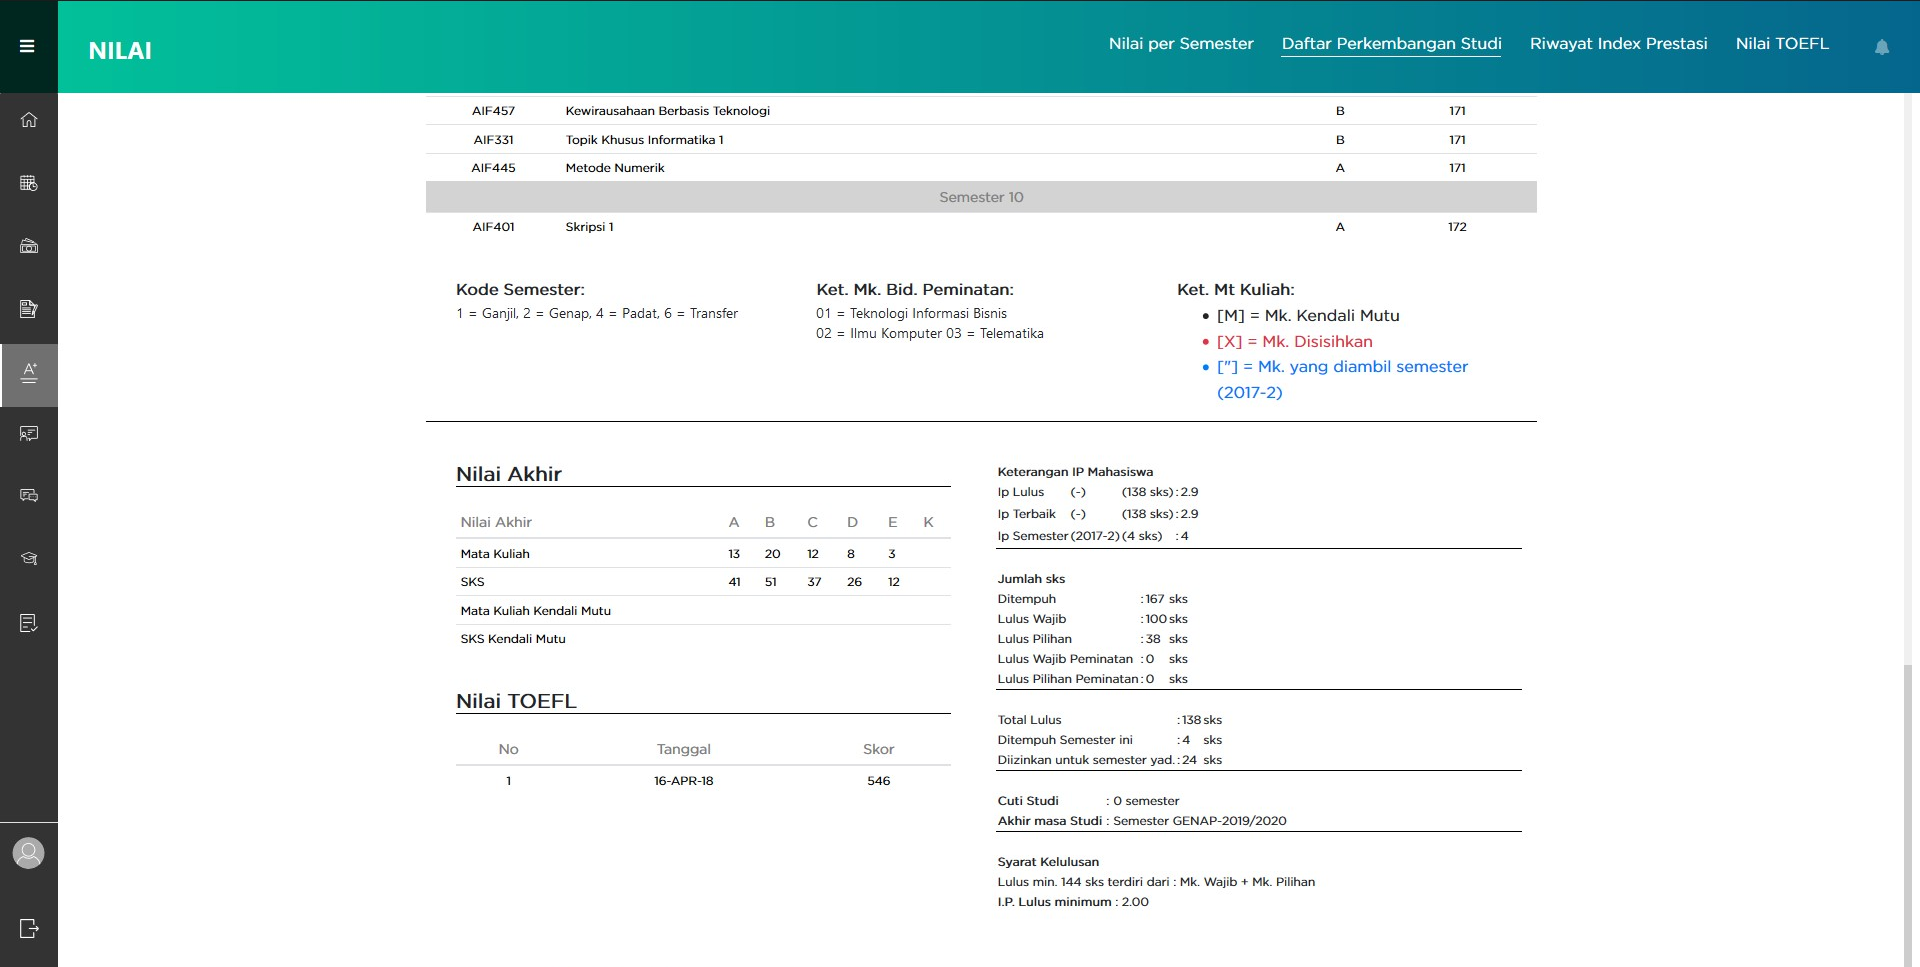
\includegraphics[scale=0.3]{Gambar/studentportal_dps_2}
				\caption{Tampilan Statistik Nilai dan IP}
				\label{fig:studentportal_dps_2}
			\end{figure}
			\item Riwayat Index Prestasi \\
			Menampilkan daftar riwayat Indeks Prestasi Semester(IPS) dan Indeks Prestasi Kumulatif(IPK) setiap semester (Gambar \ref{fig:studentportal_rip_2}). Tampilan ini juga dilengkapi dengan grafik perkembangan (Gambar \ref{fig:studentportal_rip_1})
			\begin{figure}[H]
				\centering
				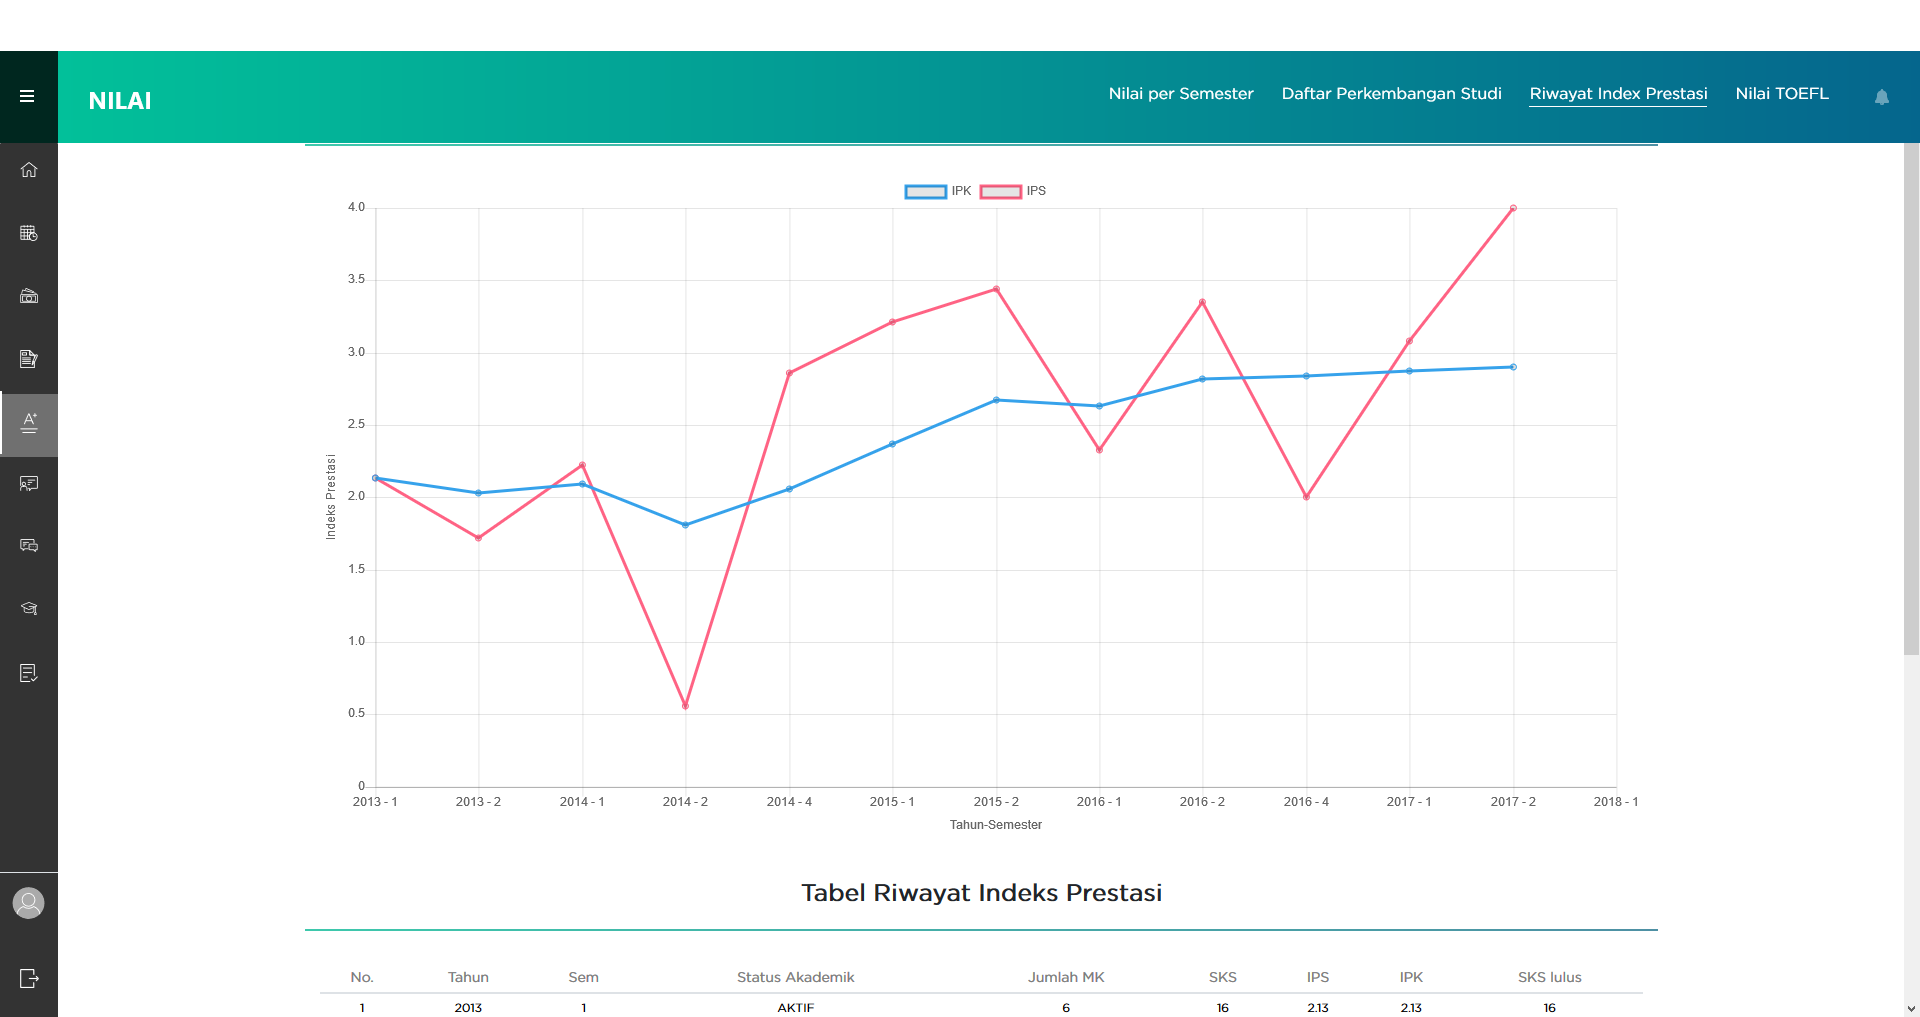
\includegraphics[scale=0.23]{Gambar/studentportal_rip}
				\caption{Tampilan Grafik Riwayat Index Prestasi}
				\label{fig:studentportal_rip_1}
			\end{figure}
			\begin{figure}[H]
				\centering
				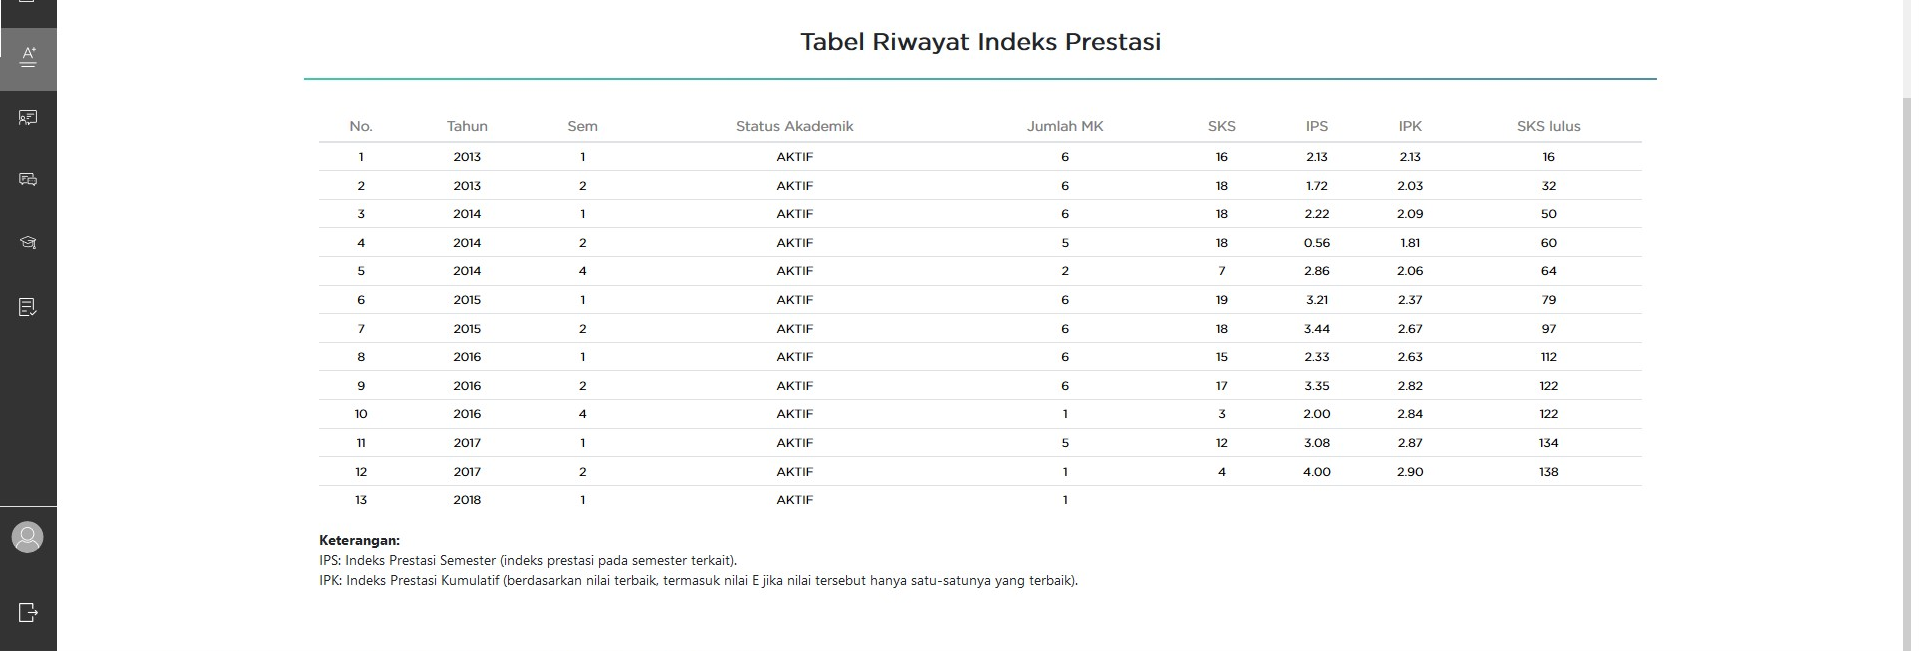
\includegraphics[scale=0.3]{Gambar/studentportal_rip_2}
				\caption{Tampilan Daftar Riwayat Indeks Prestasi}
				\label{fig:studentportal_rip_2}
			\end{figure}
			\item Nilai TOEFL \\
			Menampilkan daftar riwayat skor dan detail skor \textit{Test of English as Foreign Language} (TOEFL) yang pernah ditempuh (Gambar \ref{fig:studentportal_nilai_toefl}).
			\begin{figure}[H]
				\centering
				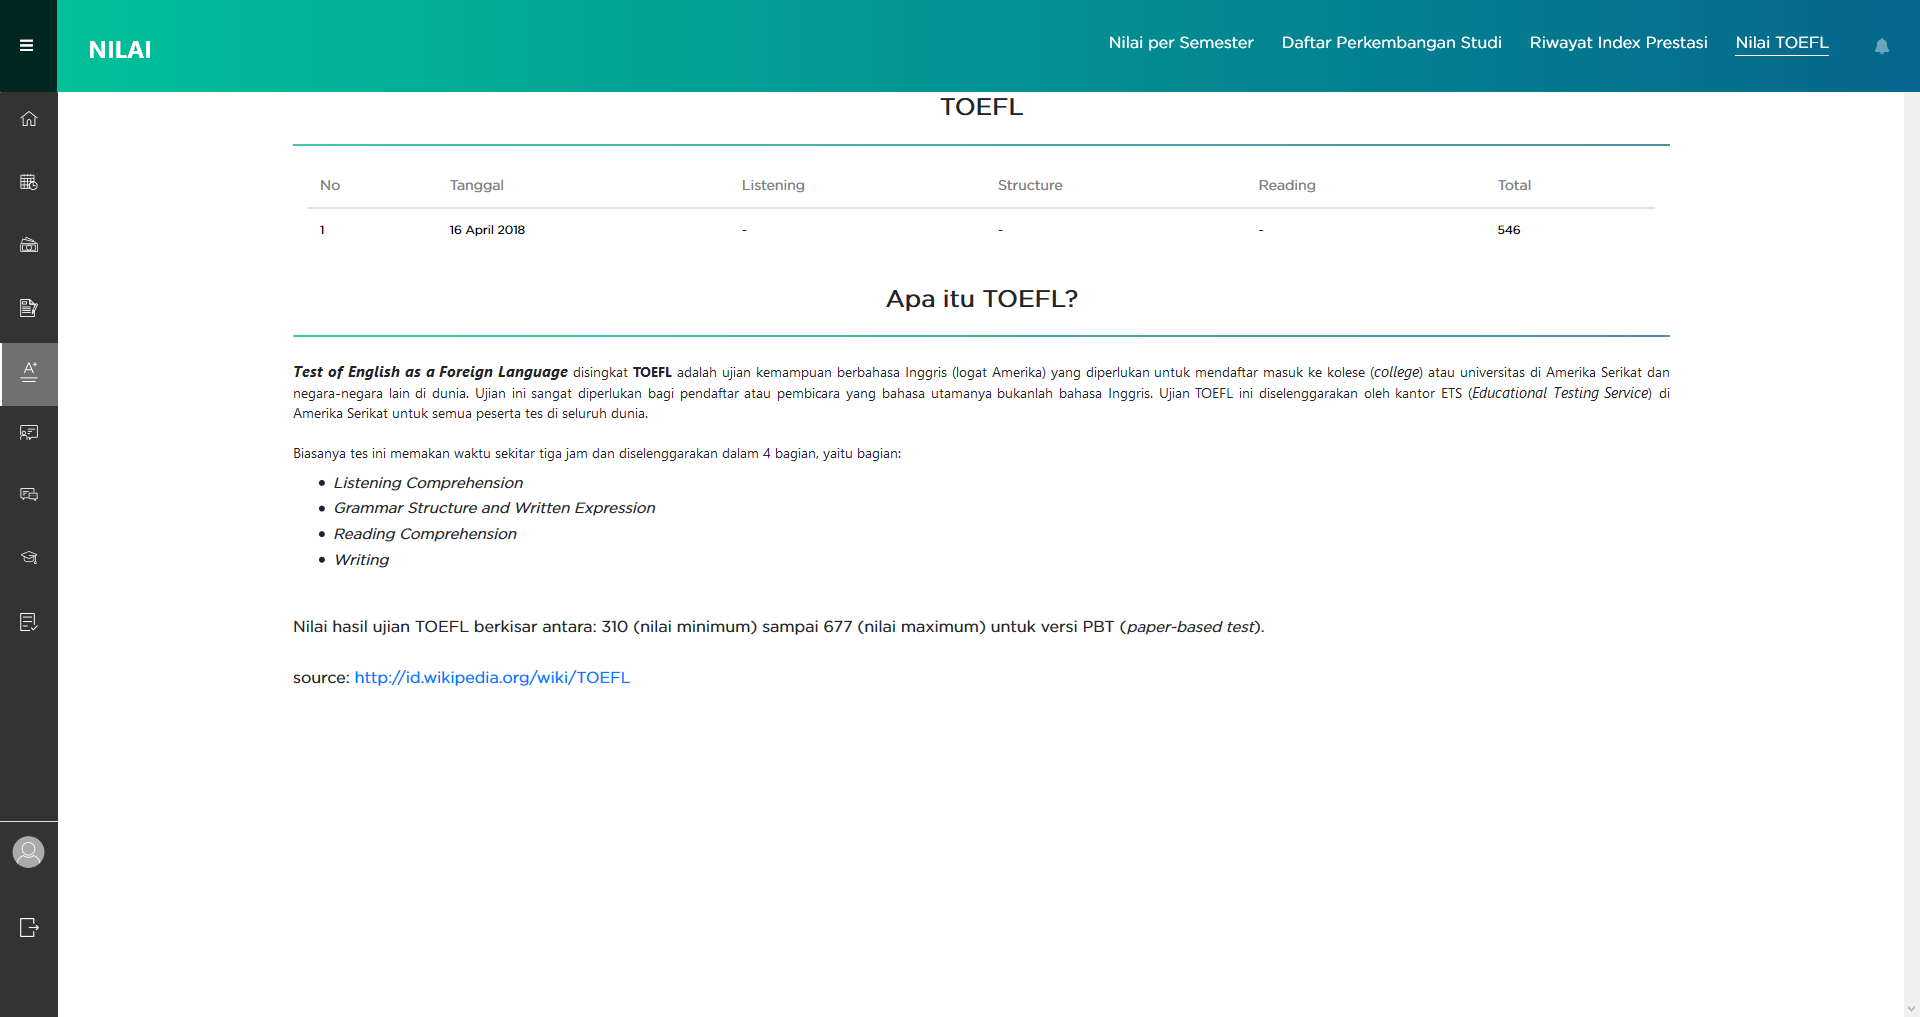
\includegraphics[scale=0.23]{Gambar/studentportal_nilai_toefl}
				\caption{Tampilan Daftar Perkembangan Studi}
				\label{fig:studentportal_nilai_toefl}
			\end{figure}
		\end{itemize}
		\item Menu Angket, Kelulusan, dan Pengajuan \\
		Menu Angket, Kelulusan, dan Pengajuan dalam tahap pembangunan.
		\item Saran dan Komentar \\
		Menu ini akan membuka link ke \url{https://suaramahasiswa.unpar.ac.id/}.
	\end{itemize}
	\item Pengumuman \\
	Menampilkan pengumuman dibagi jadi 2, yaitu pengumuman pribadi dan pengumuman prodi (Gambar \ref{fig:studentportal_pengumuman}).
	\begin{figure}[H]
		\centering
		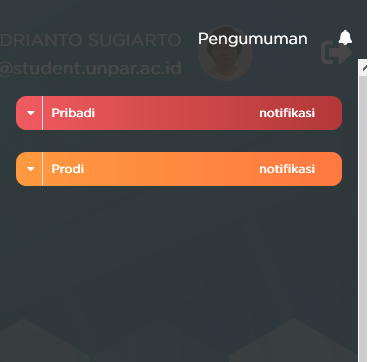
\includegraphics[scale=0.75]{Gambar/studentportal_pengumuman}
		\caption{Tampilan Pengumuman}
		\label{fig:studentportal_pengumuman}
	\end{figure}
\end{enumerate}